
\documentclass[11pt]{book}
%usepackage[italian]{babel}
\usepackage{epsfig}
%\usepackage{psfig}
\usepackage{amssymb}
\usepackage{latexsym}
\usepackage{longtable}
\usepackage{subfigure}
\usepackage{graphics}
\usepackage{lscape}
\usepackage{a4wide}

\usepackage{graphicx}
\usepackage{natbib}


\newcommand{\msun}{M$_{\odot}$}
\newcommand{\kms}{km s$^{-1}$}

\begin{document}
\begin{titlepage}
\title{{\Huge The MANGA Data Analysis Pipeline: \\
a prototype}}
\author{L. Coccato \& MANGA team}
\end{titlepage}

\maketitle
\tableofcontents

% ======================================================================
%\newcommand{\kms}{km s$^{-1}$}
%\chapter{Introduction}
%\label{dap}
%
%
%\section{Abstract}
%\label{dap_sec:abstract}%
%
%This chapter %
%
%\subsection{Acronyms and definitions}%
%
%In this chapter, we will adopt the following acronyms and definitions:
%
%\begin{tabular}{l l}
%DRP & Data Reduction Pipeline \\
%DAP & Data Analysis Pipeline \\
%LOSVD & Line Of Sight Velocity Distribution \\
%LSF & Line Spread Function \\
%SRD & Sciente Requirement Document \\
%
%
%\end{tabular}




\chapter{Introduction}
\label{dap_chap:introduction}

\section{Data Analysis Pipeline: overview}
\label{dap_sec:dap_overview}

The scope of the Data Analysis Pipeline is to analyse the output of
the Data Reduction Pipeline and deliver science products. They are
classed into two groups, the {\bf High level data products} and the
{\bf Model dependent data products}.

High level data products are:
\begin{itemize}
     \item Stellar kinematics (velocity, velocity dispersion, h3, and h4 Gauss-Hermite moments).
     \item Emission line kinematics (velocity, and velocity dispersion).
     \item Equivalent widths and fluxes of emission lines.
     \item Absorption line strengths.
     \item Reddening.
     \item Radial gradients of measured quantities.
     \item Rotation curves and kinemetric parameters.
     \item Stellar weights from full spectral fitting.
\end{itemize}

Model dependent data products are:
\begin{itemize}
    \item Stellar population parameters age, metallicity, chemical
      element ratios, and IMF, and their radial gradients (from absorption features).
    \item Stellar population parameters age, metallicity, chemical
      element ratios, and IMF, and their radial gradients (from full spectral fitting).
    \item Extinction corrected star formation rates and hystories.
    \item Gas metallicities, BPT diagrams.
    \item Mass to light ratio (from stellar population).
    \item Mass to light ratio, dynamical mass (from dynamical
      modeling).
    \item Angular momentum.
   % \item Characterization of asymmetries, see Section \ref{sec:dynamical_state}.
   % \item Measurements of the Toomre Q-parameter, see Section  \ref{sec:growth_bulges}.
\end{itemize}%



\subsection{DAP workflow description}
\label{dap_sec:dap_workflow}

The DAP is divided into parts and blocks, the first part (blocks 1-6)
will deliver the High Level Data products (see Figure
\ref{dap_fig:dap_workflow_1}), the second part (blocks 7-9) will
deliver the Model dependent data products (see Figure
\ref{dap_fig:dap_workflow_2}). 

Each block is responsable for a set of operations, such as reading
data, fitting the input spectra. The procedure that executes an
operation is called ``main module''. The main modules comunicates
between them and between the various blocks via other procedures,
which are called ``interface module''. The main and interfaces modules
can call other modules, which are called ``unitily modules''. The
interface module is therefore responsable to get input files from a
previous interface, convert them in a readable format readable for the
main module, collect the outputs of the main module and convert them
in a form readable for the next interface. In this way, it is
relatively easy to change the software responsible for a specific task
(i.e. replacing the main module responsible for the spectral fitting)
by chaning its interface.  Table \ref{dap_tab:modules} list a summary
of the blocks, interfaces and main modules distribution.

\begin{table}
\caption{Summary of blocks, interfaces and main modules distribution.}
\begin{tabular}{l |l |l }
BLOCK         & Interface modules               & Main and utility modules       \\
\hline
\hline
%{\bf Block 1} &                                 &                                \\  
              &                                 &  \\  
{\bf Block 1} & mdap\_read\_datacube            & mdap\_calculate\_spectrum\_sn  \\
\hline
%{\bf Block 2} &                                 &                                \\  
              &                                 &  \\  
{\bf Block 2} & mdap\_spatial\_binning          & mdap\_voronoi\_2d\_binning     \\
              &                                 & mdap\_calibrate\_sn            \\
\hline
%{\bf Block 3} &                                 &                                \\  
              &                                 &  \\  
{\bf Block 3} & mdap\_log\_rebin$^{1}$          & mdap\_do\_log\_rebin           \\
              &                                 & mdap\_convol\_sigma            \\
\hline
%{\bf Block 4} &                                 &                                \\  
              &                                 &  \\  
{\bf Block 4} & mdap\_spectral\_fitting$^{3}$   & mdap\_calculate\_spectrum\_sn  \\
              & mdap\_create\_starting\_guesses & mdap\_bvls                     \\
              &                                 & mdap\_dust\_calzetti           \\
              &                                 & mdap\_get\_losvd               \\
              &                                 & {\tt mpfit package}            \\
              &                                 & mdap\_sgandalf                 \\
              &                                 & mdap\_gandalf\_wrapf$^{2}$  \\
              &                                 & mdap\_gandalf$^{2}$      \\
              &                                 & mdap\_ppxf$^{2}$           \\
\hline
%{\bf Block 5} &                                 &                                         \\  
              &                                 &  \\  
{\bf Block 5} & mdap\_measure\_indices          & mdap\_read\_indices\_definitions$^{4}$  \\
              &                                 & mdap\_do\_measure\_index                \\
              &                                 & mdap\_convol\_sigma                     \\
\hline
%{\bf Block 6} &                                 &                                         \\  
              &                                 &  \\  
{\bf Block 6} & mdap\_spatial\_radial\_binning  & mdap\_calculate\_spectrum\_sn  \\
              & mdap\_spectral\_fitting$^{3}$   & mdap\_read\_indices\_definitions$^{4}$  \\                                         
              & mdap\_measure\_indices          & mdap\_do\_measure\_index                \\
              &                                 & mdap\_convol\_sigma                     \\
              &                                 & mdap\_dust\_calzetti           \\
              &                                 & mdap\_get\_losvd               \\
              &                                 & {\tt mpfit package}            \\
              &                                 & mdap\_sgandalf                 \\
              &                                 & mdap\_gandalf\_wrapf$^{2}$  \\
              &                                 & mdap\_gandalf$^{2}$      \\
              &                                 & mdap\_ppxf$^{2}$           \\
              &                                 &  \\  
\hline
              &                                 &  \\  
{\bf Block 7} &                                 &                                \\
\hline
              &                                 &  \\  
{\bf Block 8} &                                 &                                \\
\hline
              &                                 &  \\  
{\bf Block 9} &                                 &                                \\
\hline
\hline
\end{tabular}
\begin{minipage}{15cm}
Notes: 
$^{1}$ Need auxiliary files: stellar templates. 
$^{2}$ Need auxiliary file: Emission lines definitions. 
$^{3}$ It runs either mdap\_sgandalf, or the 3 routines package: mdap\_gandalf\_wrap plus
mdap\_gandalf plus mdap\_ppxf.
$^{4}$ Need auxiliary file: Absorption line index definitions.
\end{minipage}
\label{dap_tab:modules}
\end{table}

The input datacube is read in block 1 and information (vectors with
galaxy spectra, errors, wavelenght, and spatial information) are
passed to the block 2 for spatial binning. Three spatial binnings are
foreseen, depending on the scientific requirements. The current DAP
version uses the Voronoi binning scheme, (as implemented in IDL by
Cappellari \& Copin 2003), as main module for the spatial binning
task.

Binned spectra are passed to block 3 for logarithmic resampling of the
galaxy spectra (and error) and the stellar templates. Stellar
templates are also broadened to match the instrumental set up. For
this, the instrumental $LSF(\lambda)$ is required as input. Three sets
of log-sampled galaxy spectra are produced, one set for each spatial
binning.

The log-sampled spectra are then passed to block 4 for spectroscopic
measurements. Three fits are performed in block 4, one for each
spatial sampling defined in block 2. Before each fit, the log-sampled
Galaxy spectra are corrected for Milky Way extinction(input
parameter). Results from the first execution will be used to constrain
the fit of the second fit, and soforth. The current version uses i)
sgandalf.pro (a modified version of ppxf.pro by Cappellari \& Emsellem
2004, and spectral decomposition by Coccato et al. 2011); and ii)
Calzetti et al. (2000) formulas for reddening correction as main
modules in block 4 (See Section \ref{dap_sec:mdap_spectral_fitting}
for further details). The output of block 4 are the kinematic
parameters of stars and gas, emission lines fluxes and equivalent
width, reddening, the weights of the stellar templates used in the fit
(for stellar population measurements), and rest-framed galaxy spectra.

Input galaxy spectra (with best-fit emission lines removed) will be
passed to block 5 for measurement of the line strenght. The current
design foresees that absorption line strength will be measured only
onto spectra associated to the first spatial binning (i.e. those with
the higher $S/N$. The current version uses the absoprtion line indices
as defined by Worthey et al. (1994).

Rest-framed spectra, Kinematic measurements, emission line fluxes,
absorption and emission line equivalent widths are then passed to
block 6 for the extraction of the radial profiles of the measured
quantities, and kinemetric analysis.

\subsection{DAP inputs and outputs}
\label{dap_sec:dap_inputs_outputs}

The Data Analysis Pipeline consists in a IDL procedure,
manga\_dap.pro, and a set of ``interfaces'' and ``main'' modules,
which are described in this document.

To run the pipeline, the following files are needed.
\begin{itemize}

\item total\_filelist.dat. The file must contain 5 columns. The first
  column indicates the names of the $N$ datacubes (stored in .fits
  file, see Section \ref{dap_sec:mdap_read_datacube}), the second
  column provides an estimate of the galaxy redshift (in km/sec), the
  third column provides an estimate of the stellar velocity dispersion
  (in km/sec), the 4th column provides the mean galaxy ellipticity,
  and the 5th column provides the mean galaxy position angle.

\item all the $N$ datacubes listed in the file total\_filelist.dat.

\item a set of stellar templates, in fits file format (see Section \ref{dap_sec:mdap_log_rebin}).

\item emission\_lines\_setup\_with\_Balmer\_decrement. A file containing the definitions of the emission lines to include in the fit (see Section \ref{dap_sec:mdap_spectral_fittig}).

\item  absorption\_line\_indices\_definition.dat. A file containing the definitions of the absorption line indices to measure (see Section \ref{dap_sec:mdap_measure_indices}). 

\end{itemize}

The DAP is executed by the following IDL command line 

\[
{\tt IDL> manga\_dap,i,[/check\_version],[/dont\_remove\_null\_templates]}
\]
where {\tt i} is the index number of the $i$-th datacube in total\_filelist.dat, column 1 to analyse, $i=0, N-1$.

/check\_version performs the reduced version control on already
existing output data, and avoid to redude again the data if the
previous reduction is up to date.

/dont\_remove\_null\_templates By default, the DAP speeds up the
analysis by excluding some stellar templates that have zero weight
(See Section \ref{dap_sec:mdap_spectral_fitting}. If this keyword is
set, the speed up process is not activated.



 As output, the DAP returns a
multilayer fits file with all the relevant quantities (({\tt
  <datacube\_name> \_high\_level.fits}), an idl session with all the
session variables stored ({\tt
  <datacube\_name>\_mdap\_ session.idl}). These outputs are stored and
a log file (<datacube\_name>\_mdap.log) in the directory {\tt
  results/ <datacube\_name>/}, and a log file
(<datacube\_name>\_mdap.log).

The content of the {\tt <datacube\_name>\_high\_level.fits} output
file is described in Table \ref{dap_tab:output}.


\begin{center}
\begin{longtable}{p{0.5cm}|p{3.5cm}| p{10.1cm}}
\caption{Extension description of the DAP output fits file.} \label{dap_tab:output} \\
\hline
{\bf Ext} &  {\bf Name} &{\bf Description} \\
\hline
\endfirsthead
\hline
{\bf Ext} &  {\bf Name} &{\bf Description} \\
\hline
\endhead
\hline
\endlastfoot
\hline
%{\bf Ext} &  {\bf Name} &{\bf Description} \\
0 & signal              & Mean signal per pixel, produced by mdap\_read\_datacube.pro (Section \ref{dap_sec:mdap_read_datacube}). \\
1 & noise               & Mean noise per pixel, produced by mdap\_read\_datacube.pro (Section \ref{dap_sec:mdap_read_datacube}).bla bla \\
2 & binning map 1       & Location and geometry of the spatial bins of the first binning scheme.\\ 
3 & binning 1 data      & Measurements performed on the first binning scheme (absorption line indices).\\ 
4 & binning map 2       & Location and geometry of the spatial bins of the second binning scheme.\\ 
5 & binning 2 data      & Measurements performed on the second binning scheme (stellar kinematics). \\ 
6 & binning map 3       & Location and geometry of the spatial bins of the third binning scheme.\\ 
7 & binning 3 data      & Measurements performed on the third binning scheme (gas kinematics and emission line properties).\\ 
8 & binning map radial  & Location and geometry of the radial binning scheme.\\ 
9 & binning radial data & Measurements performed on the radial binning scheme (absorption line indices and stellar velocity dispersion)  \\ 
\hline
\end{longtable}
\end{center}



\subsection{Version control and tags}
\label{dap_sec:dap_version}


At the beginning of the execution, the DAP check whether the output
.fits file and .idl sessions exist. If so, it reads the version(s)
used to generate the existing files. If the current module versions
are greater than those used to generate the output file, the analysis
is performed again. 

\begin{itemize}
\item {\bf manga\_dap\_version}. The version of the DAP. If the module
  version is greater than that stored in the output files, the entire
  analysis is performed again (currently, blocks 1-5).
\item {\bf mdap\_read\_datacube\_version}. The version of modules in
  block 1. If it is greater than that stored in the output file, blocs
  1-5 are executed again.

\item {\bf mdap\_spatial\_binning\_version}. The version of modules in
  block 2. If it is greater than that stored in the output file, blocs
  2-5 are executed again. It must include version information about
  mdap\_voronoi\_binning.pro as well.

\item {\bf mdap\_log\_rebin\_version}. The version of modules in
  block 3. If it is greater than that stored in the output file, blocs
  3-5 are executed again.

\item {\bf mdap\_spectral\_fitting\_version}. The version of modules
  in block 4. If it is greater than that stored in the output file,
  blocs 4-5 are executed again. It must include version information
  about mdap\_sgandalf.pro as well.

\item {\bf mdap\_measure\_index\_version}. The version of modules in
  block 5. If it is greater than that stored in the output file, block
  5 is executed again.

\end{itemize}

Warning: the version control is enabled only if the keyword /check\_version is set.

\begin{figure}
\begin{center}
%\hspace{-2cm}
%\includegraphics[width=6cm,angle=90]{dap_workflow_1.ps}  25 150 810 445
\psfig{file=figures/mangaDAP_workflow_1.ps, width=9cm, clip=, bb= 22 20 340 800}
%\vspace*{0cm}
\caption{Workflow chart of the Data Analysis Pipeline (High Level Data products).}
 \label{dap_fig:dap_workflow_1}
\end{center}
\end{figure}


\begin{figure}
\begin{center}
%\hspace{-2cm}
%\includegraphics[width=6cm,angle=90]{dap_workflow_1.ps}  65 144 702  420 
\psfig{file=figures/mangaDAP_workflow_2.ps,  width=9cm, clip=, bb= 22 20 340 800}
%\vspace*{0cm}
\caption{Workflow chart of the Data Analysis Pipeline (Model Dependent Data products).}
 \label{dap_fig:dap_workflow_2}
\end{center}
\end{figure}

\chapter{BLOCKs and ``interface'' modules}
\label{dap_chap:blocks}
\section{DAP Block 1: reading the input data}
\label{dap_sec:block1}

This block reads the input data (in the form of a datacube or RSS
files) and extract the all information needed for further processing
such as the galaxy spectra and errors, wavelength vector, and 2D maps
containing the coordinates, and galaxy signal and noise. The interface
module in this block is: mdap\_read\_datacube.pro (see Section
\ref{dap_sec:mdap_read_datacube} for a list of inputs and outputs).

The main modules in the block, called by the interface, are
mdap\_calculate\_spectrum\_sn.pro (see Section
\ref{dap_sec:mdap_calculate_spectrum_sn} for a list of inputs and
outputs).

The Block will provide the galaxy spectra (and errors),
two-dimensional maps with coordinates (in arcseconds, the center of
the field has coordinates 0,0), the two-dimensional maps of the signal
and the noise (per angstrom), the wavelength vector (in \AA) and
related quantities (initial \AA, reciprocal dispersion
\AA\ pixel$^{-1}$), and header information for 2-dimensional
maps. Figure \ref{dap_fig:block1} illustrates the flowchart of block
1.


\begin{figure}
\begin{center}
%\hspace{-2cm}
%\includegraphics[width=6cm,angle=90]{dap_workflow_1.ps}
%\psfig{file=figures/block1.ps, width=12.0cm, clip=,bb=40 215 558 710}
\psfig{file=figures/block1.ps, width=15.0cm, clip=}
%\vspace*{0cm}
\caption{Workflow chart of the block 1 of the Data Analysis
  Pipeline. See Section \ref{dap_sec:mdap_read_datacube} for a
  description of inputs and outputs.}
 \label{dap_fig:block1}
\end{center}
\end{figure}


\subsection{{\tt mdap\_read\_datacube.pro}}
\label{dap_sec:mdap_read_datacube}

This interface module reads the input datacube or RSS files (which
must be multi-layer fits file) and extract from it all the arrays and
quantities, which are needed for the analysis. Table
\ref{dap_tab:mdap_read_datacube} list the inputs and outputs required
for this module.



\begin{center}
\begin{longtable}{p{2.7cm}| p{11.1cm}}
\caption{Inputs and outputs parameters of mdap\_read\_datacube.pro} \label{dap_tab:mdap_read_datacube} \\
\hline
{\bf  INPUTS} & \\
\hline
\endfirsthead
\hline
\endhead
\hline
\endlastfoot
\hline
datacube\_name & string with the name of the fits file containing the input in datacube or RSS formats. 
                         For inputs in datacube format, the file must be a fits file with the following
                         extensions:
                                \begin{enumerate}
                             \item flux in 1e-17 ergs/s/cm$^{-2}$/\AA. This extension must be a 3D
                               array, with the wavelength direction along the 3rd axis. 
                            \item  Inverse variance associated to the first extension
                            \item  Wavelength solution (1D dbl array). Constant linear step
                              (preferred)? Constant Log-step? Constant ln-step?
                            \item  RSS format (row-stacked spectra) (NOT USED)                  
                            \item  coverage map; (NOT USED)
                           \end{enumerate}

                         For inputs in RSS format, the file must be a fits file with the following
                         extensions:
                          \begin{enumerate}
                            \item flux in 1e-17 ergs/s/cm$^{-2}$/\AA. This extension must be a 3D
                               array, with the wavelength direction along the 3rd axis.
 
                            \item Inverse variance associated to the first extension

                            \item Wavelength solution (1D dbl array). Constant linear step
                              (preferred)? Constant Log-step? Constant ln-step?
                            
                            \item X position table.  Since position is a function of wavelength this is an 
                               array of the same size as the flux array.  Coordinates should be in arcseconds 
                               relative to the center of the data cube (i.e., roughly the center of the galaxy).
                            \item Y position table.
                            \end{enumerate}\\
%
\hline
{\bf  OPTIONAL INPUTS}  & \\
\hline
lrange & [2 elem vector]. It indicates the wavelentgh range (in angstrom) where to
       extract the information for Signal and Noise. Default: use the entire spectra range \\
%
\hline {\bf OPTIONAL KEYWORDS} &  \\ 
\hline 
/keep\_original\_ step & If set, the wavelength output vector will be the same as the one
                         define from the input fits file. The default
                         is to re-construct (and  therefore re-inrpolate the galaxy and error
                         spectra) the output wavelength vector with constant ang/pixel step
                         using the minimum ang/pixel step that is stored in the wavelength
                         solution. For MANGA data, it is suggested to set this keyword on.\\
%
 /use\_total           &   If set, the signal is the total of the counts in the selected wavelength range, the noise is the sum in
                         quadrature of the noises in the selected range. Useful for emission lines.\\
\hline
{\bf  OUTPUTS} &  \\
\hline
data           &  Galaxy spectra. [NxMxT elements array] in the case that the inputs are in datacube format, or [NxT elements array]
               in the case the inputs are in RSS format. Spectra are resampled over the vector wavelength.    \\
%
error          & Errors associated to data. [NxMxT elements array] in the case that the inputs are in datacube format, or [NxT elements array]
               in the case the inputs are in RSS format. Spectra are resampled over the vector wavelength. \\
%
wavelength     & [T elements array]. Wavalenght value (in angstrom)  where data and errors are computed. The vector is constructed with constant 
               linear step in ang/pixel 
               (unless the /keep\_original\_ step keyword is selected). If input spectra have a logarithmic sampling, 
               the minimum available step is used (e.g. log\_lam[1]-log\_lam[0], converted into angstrom).  In the case of MANGA data, 
               we recommend to set the /keep\_original\_ step keyword, to have the wavelength output vector equal to the wavelength vector of the data.\\
%
x2d            & Array containing the x coordinates in arcseconds (0 is the center of the field of view). 
               [NxM elements array] in the case that the inputs are in datacube format, or 
               [N elements array] in the case the inputs are in RSS format. \\
%
y2d            & Array containing the y coordinates in arcseconds (0 is the center of the field of view). 
               [NxM elements array] in the case that the inputs are in datacube format, or 
               [N elements array] in the case the inputs are in RSS format. \\
%
signal         & Mean galaxy signal per \AA, obtained considering all the wavelength range 
               (or only the range specified by lrange), for each input spectrum.               
               [NxM elements array] in the case that the inputs are in datacube format, or 
               [N elements array] in the case the inputs are in RSS format. 
               The signal is computed as the median of each spectrum, in the wavelength range specified by lrange (unless the keyword /use\_total is set). \\
\\
%
noise          & Mean galaxy error per \AA, obtained considering all the wavelength range 
               (or only the range specified by lrange)), for each input spectrum. Calculation is done on original spectra, not 
               those resampled over the vector wavelenght.
               [NxM elements array] in the case that the inputs are in datacube format, or 
               [N elements array] in the case the inputs are in RSS format.
               The signal is computed as the median of each error, in the wavelength range specified by lrange (unless the keyword /use\_total is set).\\
%               
cdelt1         & [double].        Spatial sampling along x direction (arcsec/pixel). If inputs are in RSS format, it is set to 0.5 arcsec/pixel.  \\
%               
cdelt2         & [double].        Spatial sampling along y direction (arcsec/pixel). If inputs are in RSS format, it is set to 0.5 arcsec/pixel.  \\
%               
header2d       & [str array].     The header for output two-dimensional maps produced by the DAP. \\
\hline
{\bf  OPTIONAL OUTPUTS} &  \\
\hline
%
 x2d\_ reconstructed  &   [NxM] elements array]   if input is in DATACUBE format,  and x2d\_ reconstructed = x2d.

                          [N'xM'] elements array] if inputs are in RSS format, the x2d coordinates are resampled over a 2D map with fixed 0"5/pixel sampling
                                     and define the  x2d\_ reconstructed map.\\
%
 y2d\_ reconstructed &    [NxM] elements array   if input is in DATACUBE format,  and y2d\_reconstructed = y2d.

                          [N'xM'] elements array if inputs are in RSS format, the y2d coordinates are resampled over a 2D map with fixed 0"5/pixel sampling
                                     and define the  y2d\_ reconstructed map.\\
%
 signal2d\_ reconstructed  &  [NxM] elements array if input is in DATACUBE format, and  signal2d\_reconstructed = signal.

                         [N'xM'] elements array if inputs are in RSS format, the signal is resampled over the 2D map defined by
                                         x2d\_ reconstructed  and y2d\_ reconstructed. \\
%
 noise2d\_ reconstructed  &   [NxM] elements array if input is in DATACUBE format, and noise2d\_reconstructed = noise.

                        [N'xM' array] If inputs are in RSS format, the noise is resampled over the 2D map defined by
                                         x2d\_reconstructed  and y2d\_reconstructed. \\
%
 version   & [string]            Module version. If requested, the module is not execute and only version flag is returned.\\
%
\hline
\end{longtable}
\end{center}

Note: NaN values in each error vector will be replaced by the median
error value (computed using error's defined values).


\subsubsection{Future developments}

The following items needs to be implemented:

\begin{itemize}
  \item Implement with new format of input datacube (i.e. read and handlemask arrays).
  \item Allow for identification and removal of foreground stars.
  \item Get Milky Way extinction, and provide extinction-corrected galaxy spectra and errors. 
        Insert an appropriate main module (i.e. dust\_getval.pro) to do this
  
\end{itemize}




\section{DAP Block 2: Spatial binning}

This block adds adjacent spectra in the field of view to reach a
minimum signa-to-noise ratio, and organizes the observations into
spatial bins. 

It requires the spectra, errors, signals and noise for each spectrum,
and the coordinates obtained from block 1 as inputs. It returns the
binned spectra (and errors) and all the geometrical information of the
spatial bin (2D maps and coordinates of the bins center). It handles
both datacubes and RSS input files format.

Three different spatial binning schemes with different
are handled, depending on the scientific purposes.


\begin{enumerate}

\item First binning, which requires a minimum $S/N = 40$ per
  pixel. The spectra binned this way will be used to measure the
  equivalent width ob absorption line indices, to perform the full
  spectral fitting, and to derive the stellar population properties.

\item Second binning, which requires a minimum $S/N = 25$ per
  pixel. The spectra binned this way will be used to measure the
  stellar kinematics and dynamical models.


\item Third binning, which requires a minimum $S/N = 15$ per
  pixel. The spectra binned this way will be used to measure the
  emission line kinematics, fluxes, and widths, the reddening, gas
  metallicities and star formation rates.

\end{enumerate}

 $S/N$s are computed in the wavelength range $5560 < \lambda < 6942$
(SLOAN r-band).  The interface module in this block is
mdap\_spatial\_binning.pro (see Section
\ref{dap_sec:mdap_spatial_binning}). The main modules are:
mdap\_voronoi\_2d\_binning.pro (Section
\ref{dap_sec:mdap_voronoi_2d_binning}) and mdap\_calibrate\_sn.pro
(Section \ref{dap_sec:mdap_calibrate_sn}).


mdap\_voronoi\_2d\_binning.pro uses an imlementation of the Voronoi
Binning technique developed by \citet{Cappellari+03} (see Section
\ref{dap_sec:mdap_voronoi_2d_binning}). The implementation accounts
for spatial correlation between errors of adjacent spectra: the
estimated $S/N$ is calibrated to the real $S/N$ via empirical relation
and it is done by the main module mdap\_calibrate\_sn.pro.

Note that RSS spectra do not require the above $S/N$ calibration,
because the errors between adjacent RSS files are not correlated.

Figure \ref{dap_fig:block2} illustrates the flowchart of
block 2.

\subsubsection{future implementations}
Possible implementations are:

\begin{itemize}

\item  include the possibility to perform a radial and azimuthal
  binning, regardless of the signal-to-noise.
 \item calculation of spatial covariance matrix to account for error
   correlations and avoid the use of $S/N$ calibration relations.
\end{itemize}

\begin{figure}
\begin{center}
%\hspace{-2cm}
%\includegraphics[width=6cm,angle=90]{dap_workflow_1.ps}
\psfig{file=figures/block2.ps, width=16.0cm, clip=,bb=42 77 590 797}
%\vspace*{0cm}
\caption{Workflow chart of the block 2 of the Data Analysis
  Pipeline.}
 \label{dap_fig:block2}
\end{center}
\end{figure}

\subsection{{\tt mdap\_spatial\_binning.pro}}
\label{dap_sec:mdap_spatial_binning}

This module is an interface for the mdap\_voronoi\_2d\_binning.pro
module, which uses the Voronoi Binning scheme (modified Loyd
algorithm) to combine adjacent spectra in the field of view till a
minimum $S/N$ is reached (see Section
\ref{dap_sec:mdap_voronoi_2d_binning}).

If the minimum $S/N$ is not reached, the requirement will be
automatically decreased by a factor 0.7 till convergence. By default,
spectra with mean $S/N < 4$ per \AA will be discarded. At least, 1
spectrum per datacube will be produced.

If user-defined spatial binning is provided (via the user\_bin\_map
keyword) the Voronoi binning scheme is overrided.

Table \ref{dap_tab:mdap_spatial_binning} lists the inputs and outputs
required for this module.

\begin{center}
\begin{longtable}{p{2.7cm}| p{11.1cm} }
\caption{Inputs and outputs parameters of mdap\_spatial\_binning.pro} \label{dap_tab:mdap_spatial_binning} \\
\hline
\endfirsthead
\hline
\endhead
\hline
\endlastfoot
\hline
{\bf  INPUTS} & \\
\hline
data   &    Galaxy spectra as produced by mdap\_read\_datacube.pro.
           [NxMxT dbl array] if DATACUBE format or [NxT dbl array]if RSS format.\\
%
error  &    Errors associated to data, produced by mdap\_read\_datacube.pro.
           [NxMxT dbl array] if DATACUBE format or [NxT dbl array]if RSS format.\\
%
signal  &   Mean galaxy signal per \AA, produced by mdap\_read\_datacube.pro.
           [NxM dbl array] if DATACUBE format or [N dbl array]if RSS format.\\
%
noise  &    Mean galaxy error per \AA,  produced by mdap\_read\_datacube.pro. 
           [NxM dbl array] if DATACUBE format or [N dbl array]if RSS format.\\
%
min\_sn &    [float] Minimum S/N (per \AA) required for the output binned spectra.\\
%
x2d   &     Array containing the x coordinates in arcseconds (0 is the center of the field of view), produced by  mdap\_read\_datacube.pro.    
            [NxM dbl array] if DATACUBE format or [N dbl array]if RSS format.\\
%
y2d   &     Array containing the y coordinates in arcseconds (0 is the center of the field of view), produced by  mdap\_read\_datacube.pro.    
           [NxM dbl array] if DATACUBE format or [N dbl array] if RSS format.\\
%
stepx  &    [float] Scale arcsec/pixel along X direction, computed by  mdap\_read\_datacube.pro. \\
%
stepy   &   [float] Scale arcsec/pixel along Y direction, computed by  mdap\_read\_datacube.pro. \\
%
\hline
{\bf OPTIONAL INPUTS} & \\
\hline
%
sn\_thr   &  [float] If specified, spectra with S/N lower than this value will be excluded from the analysis. \\ 
%
x2d\_ reconstructed & [N'xM' array] Two-dimesional map of X coordinates where the output spatial\_binning should be created. Required and used only  
                    if the input data are in RSS format. \\
%
y2d\_ reconstructed & [N'xM' array] Two-dimesional map of Y coordinates where the output spatial\_binning should be created. Required and used only 
                    if the input data are in RSS format. \\
%
SN\_ CALIBRATION    & vector. If provided, the estimated signal-to-noise ({\tt SN\_est}) is converted into the real signal-to-noise ({\tt SN\_real}) using the empirical
                  calibration function defined in mdap\_calibrate\_sn.pro:
           \[
           {\rm S/N_{REAL}} = \sum_{i=1,N} C_i \cdot \left( \frac{{\rm S/N_{ESTIMATED}}^{C_0}}{ \sqrt{{\rm N}_{\rm spax} }} \right)^{i-1} 
            \]

                    where {\tt Nbin} is the number of spectra added in that spatial bin.\\
%
user\_bin\_map   &  string  If provided, the spatial map will be created
                      from the fits fiel specified by this input. The
                      fits file must contain the CRVAL1, CRVAL2,
                      CDELT1, CDELT2, NAXIS1, NAXIS2, CRPIX1, and
                      CRIX2 header keywords (coordinate units in
                      arcseconds, 0,0 indicates the center of the
                      field of view. \\

\hline
{\bf INPUT KEYWORDS} & \\
\hline
%
/plot        &       If set, some plots on X11 terminal will be shown. Not suggested if the task is launched remotely. \\
% 
/weight\_for\_sn & If set, the spectra in the same spatial bin will be
                 weighted by $S/N^2$ before being added. If The voronoi binning scheme
                 is adopted, the S/N in the bin is computed via equation (3) of
                 Cappellari \& Copin (2003) and the centers of te spatial bins are computed by
                 weighting spectra coordinates by $S/N^2$.\\ 
%
\hline
{\bf OUTPUTS} & \\
\hline
%
binning\_map & Two dimensional map showing the binning sheme. Pixels beloning to the i-th bin have value i (i=0, 1, ..., Nbins). 
             Pixels associated to no spatial bin have value -1.  
             [NxM dbl array] if inputs are in DATACUBE format or [N'xM' dbl array] if inputs are in RSS format (interpolated 
             over x2d\_reconstructed and y2d\_reconstructed).\\
%
spectra   &  [Nbins x T dbl array]    The binned spectra of the spatial Nbins. i-th spectrum is associated to the i-th bin. \\
%
errors    &  [Nbins x T dbl array]    Errors vectors associate do the binned spectra. \\
%
xNode     &  [Nbins elements array]   X-Coordinates in arcsec of the luminosity weighted centers of the spatial bins. \\
%
yNode     &  [Nbins elements array]   Y-Coordinates in arcsec of the luminosity weighted centers of the spatial bins. \\
%
area\_bins &  [Nbins elements array]   Area (in arcsec$^2$) of each spatial bin.  \\
%
bin\_sn   &  [Nbins elements array]   Mean S/N per \AA reached in each spatial bin. \\
%
\hline
{\bf OPTIONAL OUTPUTS} & \\
\hline
%
 nelements\_ within\_ bin & [Nbins elements array] number of spaxels (in the case of DATACUBE format) or number of fibres (in the case of RSS format) coadded in each spatial bin.\\
%
 version   & [string]            Module version. If requested, the module is not execute and only version flag is returned.\\
\hline
\end{longtable}
\end{center}




\section{DAP Block 3: Logarithmic sampling of input galaxy spectra and stellar templates}

This block is responsable for:

\begin{itemize}

\item resampling the input galaxy spectra and errors (rebinned
  spectra, input from block 2) to a ln-wavelength constant step.

\item resampling the stars in the spectral library in the same
  ln-wavelength constant step used for galaxy spectra, and ensuring
  that the stars have the same instrumental resolution (i.e. the same
  LSF) of the galaxy spectra.

\item selecting only the wavelength region of interest, making sure
  that the wavelenght range of the template stars is larger than that
  of the galaxy spectra.

\item defyning the wavelenght vectors (ln units) over which the galaxy
  spectra, galaxy errors, and template stars are defined.

\end{itemize}

Because the DAP performs three different spatial binnings of the input
galaxy, the block operates

The interface module in this block is mdap\_log\_rebin.pro (see
Section \ref{dap_sec:mdap_log_rebin}), which calls the main module
mdap\_do\_log\_rebin.pro that performs the logarithmic resampling (see
Section \ref{dap_sec:mdap_do_log_rebin}). Because the DAP performs
three different spatial binnings of the input galaxy, block 3 executes
mdap\_log\_rebin.pro three times, one for each set of spatially binned
spectra. The workflow of block 3 is shown in Figure
\ref{dap_fig:block3}.

The current version of the DAP uses the MARCS stellar library models
(Maraston \& Stromback, 2011, MNRAS, 418, 2785).

\begin{figure}
\begin{center}
%\hspace{-2cm}
%\includegraphics[width=6cm,angle=90]{dap_workflow_1.ps}
\psfig{file=figures/block3.ps, width=13.5cm, clip=,bb=30 70 592 790}
%\vspace*{0cm}
\caption{Workflow chart of the block 3 of the Data Analysis
  Pipeline.}
 \label{dap_fig:block3}
\end{center}
\end{figure}

\subsection{{\tt mdap\_log\_rebin.pro}}
\label{dap_sec:mdap_log_rebin}

This interface controls the main module is responsable for the
logarithmic resampling of the input galaxy spexctra, errors, and the
stellar templates. It also broadens the input stellar spectra to match
the galaxy instrumental resolution. 

The list of input/output parameters defined in mdap\_log\_rebin.pro is
given in Table \ref{dap_tab:mdap_log_rebin}.



\begin{center}
\begin{longtable}{p{2.7cm}| p{11.1cm}}
\caption{Inputs and outputs parameters of mdap\_log\_rebin.pro} \label{dap_tab::mdap_log_rebin} \\
\hline
\endfirsthead
\hline
\endhead
\hline
\endlastfoot
\hline
{\bf  INPUTS} &  \\
\hline
spectra   &   [NxT dbl array].  The N galaxy spectra to resample.\\
%
errors    &   [NxT dbl array].  Errors associated to the N spectra.\\
%
wavelength & [dbl array].     Array with T elements, that specifies the wavelengths where galaxy spectra and errors are defined.\\
%
library    &  [string].          Directory containing the template spectra. Template spectra must be in fits format, defined over a 
                             linear wavelength with constant ang/pix step, and must contain all the header information needed to  
                             recover the wavelenght domain (i.e. CRPIX1, CDELT1, and CRVAL1).\\
%
fwhm\_diff &   [dbl array].     Vector containing the FWHM(lambda) that the stellar spectra must be convolved for. At the moment, 
                             the value median(fwhm\_diff/wavelength*c) is used for broadening. Implementation to use the full 
                             LSF(lambda) information are foreseen.\\
%
\hline
{\bf  OPTIONAL INPUTS} & \\
\hline
input\_velscale & [flt].    Constant km/sec/pixel to be used when rebinning the input spectra. If not provided, the value will be
                             automatically set by the procedure.\\
%
wave\_range  & [2 elem array].   If specified, the galaxy spectra will be trimmed to this wavelength range (units: angstrom). Default: 
                             use the entire input wavelength range. Stellar spectra will be trimmed by 
                             wave\_range[0] - 250 ang and wave\_range[1] + 250 ang.\\

%
\hline
{\bf  OPTIONAL KEYWORDS}  & \\
\hline
/flux    &                  If set, flux conservation is applied to the log resampling. **Do not use** for template fitting.\\
/gal\_wavelength\_ log\_step &  Set this keyword if the input galaxy spectra are logarithmically sampled (i.e. wavelength has a logarithmic progression).\\
/quiet    &                    If set, message prompt is suppressed.\\
\hline
{\bf  OUTPUTS} &  \\
\hline
%
log\_spc  &  [N x TT dbl array]. The logarithmically resampled (ln-lambda) N galaxy spectra, over the wavelength range ln(wave\_range).\\
%
log\_err &   [N x TT dbl array]  The errors associated to the log\_spc. Errors are rebinned using the following formulas:


                              \ \ \   lrg=minmax(wavelength)

                              \ \ \   mdap\_do\_ log\_rebin, lrg, errors$^2$, log\_err2, loglam, velscale=velscale

                              \ \ \  log\_err = $\sqrt{{\rm log\_err2}}$

                             where mdap\_do\_log\_rebin.pro is the original procedure by M. Cappellari (see
                             Section \ref{dap_sec:mdap_do_log_rebin}).\\
%
log\_wav &   [TT dlb array].    The values of the ln-lambda over which log\_spc and log\_err are defined.\\
%
library\_log & [W x M dbl array]. The W stellar template spectra, logarithmically resampled.\\
%
log\_wav\_ library &[M dbl array]. The values of log-lambda over which the stellar templates are defined.\\
\hline
{\bf  OPTIONAL OUTPUTS} &  \\
\hline
version & string specifying the module version. If requested, the module is not execute and only version flag is returned.\\
\hline
\end{longtable}
\end{center}


\section{DAP Block 4: Spectral fitting}

This block is responsable for fitting the input galaxy spectra with a
set of stellar templates and Gaussian Emission lines to derive the
kinematics of stars, ionized gas, and emission line fluxes and
equivalent widths.

The main modules in this block are mdap\_spectral\_fitting.pro (see
Section \ref{dap_sec:mdap_spectral_fitting}), mdap\_get\_2d\_ map.pro
(see Section \ref{dap_sec:mdap_get_2d_map}), and
mdap\_create\_starting\_guesses.pro (see Section
\ref{dap_sec:mdap_create_starting_guesses}).

The module mdap\_spectral\_fitting.pro is an interface, that arranges
inputs and outputs for the routine that performs the actual fit, i.e.
mdap\_sgandalf.pro (called by mdap\_spectral\_ fitting.pro), which is
an improved version of the pPXF routine by \citet{Cappellari+04} (see
Section \ref{dap_sec:mdap_sgandalf} for information on how the fit is
performed).

The block executes the module mdap\_spectral\_fitting.pro three times,
once for each set of spatially binned spectra.  The current version of
the DAP uses the MARCS stellar library models (Maraston \& Stromback,
2011, MNRAS, 418, 2785) for the spectral fitting.



\begin{enumerate}

\item {\it First module execution.} The log-sampled Galaxy spectra are
  fitted with a linear combination of stellar templates and Gaussian
  Emission lines. This step requires input starting guesses of the
  galaxy redshift and stellar velocity dispersion (more than one
  redshift, and coordinates of galaxy centers if more galaxies are
  presented in the field of view). The galaxy spectra with the
  best-fit emission lines removed produced as output will be used to
  measure the absorption line strenghts (block 5). If the Milky-Way
  extinction value is provided, the input galaxy spectra are corrected
  before fitting. Galaxy reddening is also fitted, if required. This
  execution does not provide final highlevel data products, but it will
  provides: i) galaxy spectra with the best-fit emission lines removed
  (which will be used in block 5 to measure the absorption iline
  indices), ii) the weights of the stellar templates (which will be
  used to compute the stellar populations in block 7).
  
\item {\it Second module execution.} The results of the first
  execution (stellar and emission lines kinematics) are re-sampled
  over the second spatial sampling and used as starting guesses for
  the second execution on the second set of galaxy spectra (second
  spatial binning). This step is performed by the modules
  mdap\_get\_2d\_map.pro (Section \ref{dap_sec:mdap_get_2d_map}) and
  mdap\_create\_starting\_guesses.pro (Section
  \ref{dap_sec:mdap_create_starting_guesses}). As in the first
  execution, log-sampled Galaxy spectra are fitted with a linear
  combination of stellar templates and Gaussian Emission lines. Only
  those stellar templates that are selected in the first execution,
  will be used in the second run (unless the keyword
  /dont\_remove\_ null\_templates of the manga\_dap is set, see
  Section \ref{dap_sec:dap_inputs_outputs}). If the Milky-Way extinction value is provided,
  the input galaxy spectra are corrected before fitting. The final
  high level products produced in this execution are the stellar
  kinematics (V,$\sigma$, H3, and H4).

\item {\it Third module execution.} The emission line kinematics from
  the second execution are re-sampled over the third spatial sampling
  and used as starting guesses for the third execution. The stellar
  kinematics from the second execution are re-sampled over the third
  spatial sampling and {\it fixed} in the third execution.  The
  spatial resampling step is performed by the modules
  mdap\_get\_2d\_map.pro (Section \ref{dap_sec:mdap_get_2d_map}) and
  mdap\_create\_starting\_guesses.pro (Section
  \ref{dap_sec:mdap_create_starting_guesses}). As in the first
  execution, log-sampled Galaxy spectra are fitted with a linear
  combination of stellar templates and Gaussian Emission lines. Only
  those stellar templates that are selected in the first execution,
  will be used in the third run (unless the keyword
  /dont\_remove\_ null\_templates of the manga\_dap is set, see
  Section \ref{dap_sec:dap_inputs_outputs}). If the Milky-Way extinction value is
  provided, the input galaxy spectra are corrected before fitting. The
  final high level products produced in this execution are: the
  emission line kinematics (V,$\sigma$), reddening, and fluxes and
  equivalent widths (reddening corrected).

\end{enumerate}

Block 4 requires as input the log-resampled spectra of the galaxy (and
errors) and the stars, wavelenght vectors, the binning spatial
informations, and starting guesses for the galaxy redshift and
velocity dispersion.

At the end of block 4, the two-dimensional fields of stellar
kinematics (V, $\sigma$, h3, and h4) emission line kinematics (V,
$\sigma$), emission line fluxes and equivalent widths, and stellar
template weights for each of the spatial binning scheme are
provided. A two-dimensional map of the reddening is also computed for
the first and third spatial binning scheme. Best fit spectra are also
produces as output, in the rest frame wavelength or in the observed
wavelength frame, according to the user's input request.

Figures \ref{dap_fig:block4} and \ref{dap_fig:block4a} shows the
flowchart of block 4.

\begin{figure}
\begin{center}
%\hspace{-2cm}
%\includegraphics[width=6cm,angle=90]{dap_workflow_1.ps}
\psfig{file=figures/block4.ps, width=16cm, clip=}
%\vspace*{0cm}
\caption{Workflow chart of the block 4 of the Data Analysis Pipeline.}
 \label{dap_fig:block4}
\end{center}
\end{figure}


\begin{figure}
\begin{center}
%\hspace{-2cm}
%\includegraphics[width=6cm,angle=90]{dap_workflow_1.ps}
\psfig{file=figures/block4.ps, width=13.5cm, clip=,bb=40 1060 1300 1950}
%\vspace*{0cm}
\caption{Workflow chart of the block 4 of the Data Analysis Pipeline,
  zoom around the first fit section.}
 \label{dap_fig:block4a}
\end{center}
\end{figure}


\section{DAP Block 5: Measurement of absorption line indices}
\label{dap_sec:block5}

This module is responsible for measuring the equivalent width of
absorption line indices on the galaxy spectra where the best fit model
for emission lines has been removed.

It requires the following inputs:
\begin{itemize}
 
\item The galaxy spectra with emission lines removed (from block 4).

\item The stellar velocity.

  \item The LSF as function of wavelenght (to a proper
broadening of the input spectra to the reference calibration system,
e.g. Lick, MILES).

\item The best fitting stellar template and the best fitting stellar
  template convolved by the best fitting LOSVD, for intrinsic
  broadening correction (from block 4).

\end{itemize}

Figure \ref{dap_fig:block5} illustrates the flowchart of this block.

The main module in this block is mdap\_measure\_ indices.pro (see
Section \ref{dap_sec:mdap_measure_indices}), which calls the procedure
that performs the measurement mdap\_do\_ measure\_index.pro (see
Section \ref{dap_sec:mdap_do_measure_index.pro}).

Figure \ref{dap_fig:block5} illustrates the flowchart of the main module in this block.

\begin{figure}
\begin{center}
%\hspace{-2cm}
%\includegraphics[width=6cm,angle=90]{dap_workflow_1.ps}
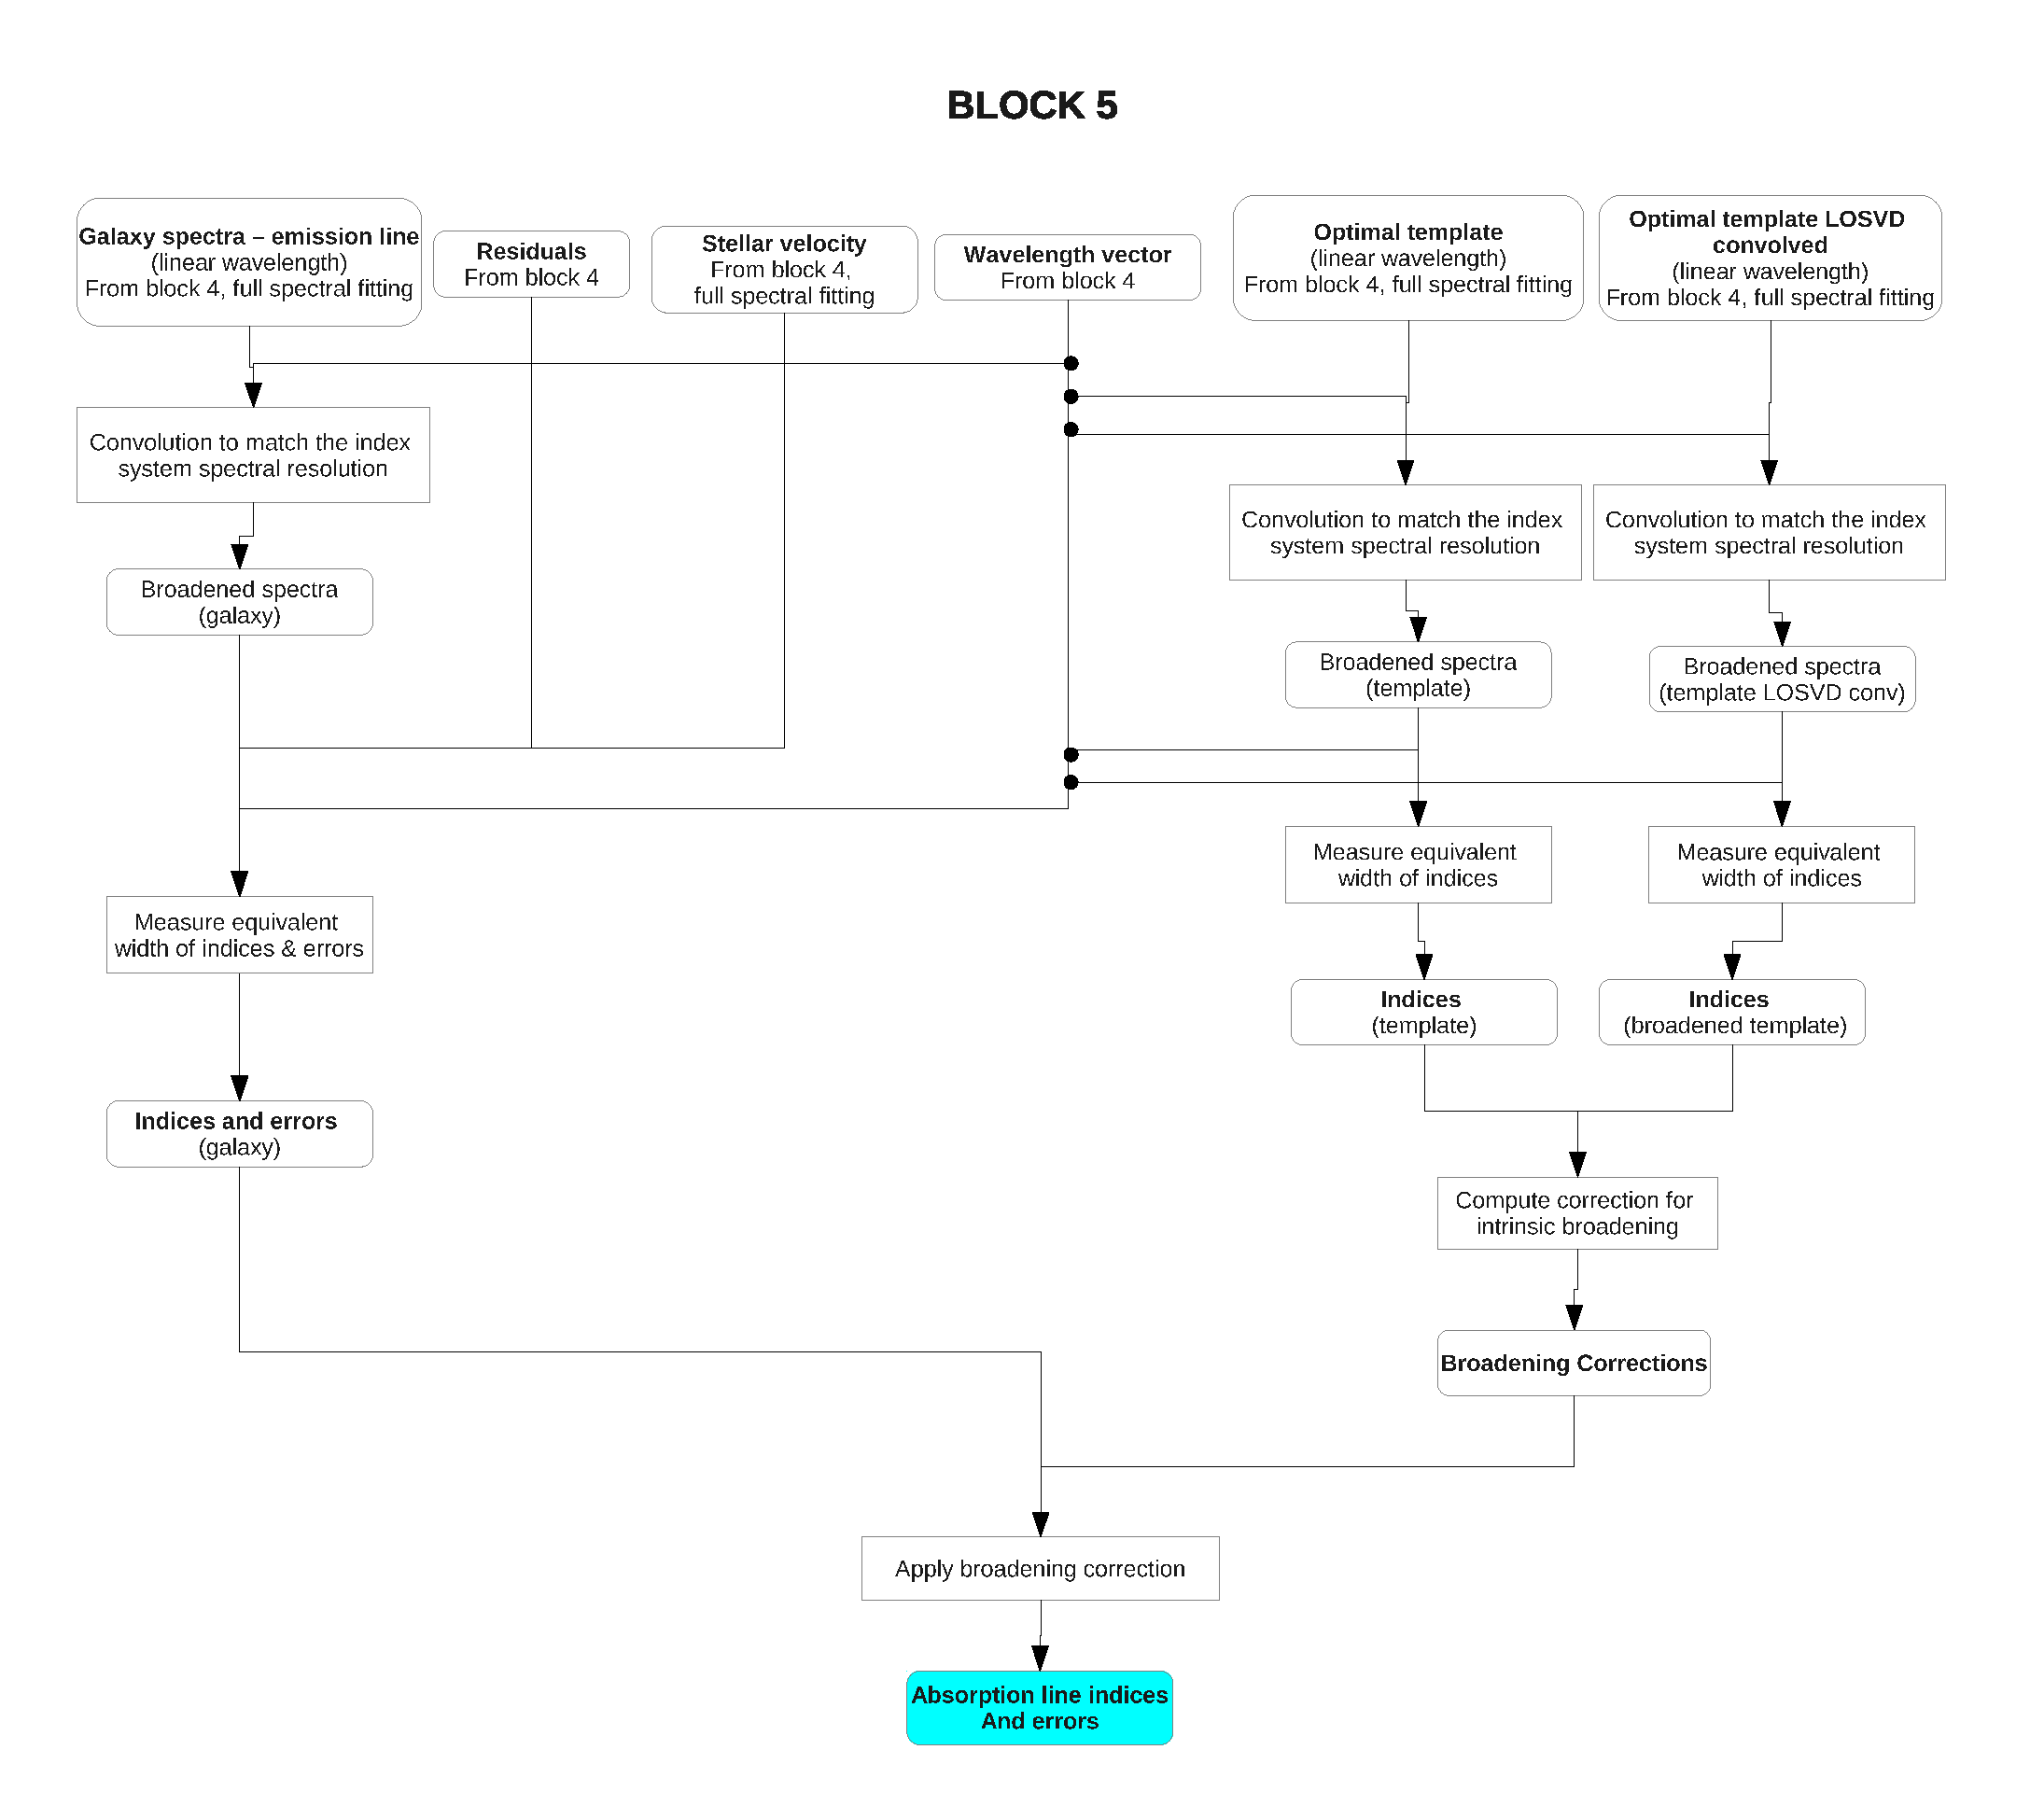
\psfig{file=figures/block5.ps, width=13.5cm, clip=}
%\vspace*{0cm}
\caption{Workflow chart of mdap\_measure\_indices.pro, the main module in block 5 of the Data Analysis Pipeline.}
 \label{dap_fig:block5}
\end{center}
\end{figure}



\section{DAP Block 6: Radial properties of high level data products}
T.B.D.

\section{DAP Block 7: Stellar population analysis}
T.B.D.

\section{DAP Block 8: Properties of the emission lines}
T.B.D.

\section{DAP Block 9: Mass modeling}
T.B.D.


\chapter{Main modules}
\label{dap_chap:dap_modules}

In this Dection we describe the individual modules in the DAP.

\section{{\tt mdap\_calculate\_spectrum\_sn.pro}}
\label{dap_sec:mdap_calculate_spectrum_sn}

bla bla bla

\section{{\tt mdap\_voronoi\_2d\_binning.pro}}
\label{dap_sec:mdap_voronoi_2d_binning}

This procedure is taken from the Voronoi Binning procedure by
Cappellari \& Copin (2003).  It has been modified so it automatically
relaxes the minimal $S/N$ requirements to have at least 1 bin in the
field of view. Table \ref{dap_tab:mdap_voronoi_2d_binning} lists the
inputs and outputs required for this module.


\begin{center}
\begin{longtable}{p{2.7cm}| p{11.1cm}}
\caption{Inputs and outputs parameters of mdap\_voronoi\_2d\_binning} \label{dap_tab:mdap_voronoi_2d_binning} \\
\hline
\endfirsthead
\hline
\endhead
\hline
\endlastfoot
\hline
{\bf  INPUTS} &  \\
\hline
X &[flt array] Vector containing the X coordinate of the pixels to bin.
             Arbitrary units can be used (e.g. arcsec or pixels).
            In what follows the term ?pixel? refers to a given
            spatial element of the dataset (sometimes called ?spaxel? in
            the IFS community): it can be an actual pixel of a CCD
            image, or a spectrum position along the slit of a long-slit
            spectrograph or in the field of view of an IFS
            (e.g. a lenslet or a fiber).
            It is assumed here that pixels are arranged in a regular
            grid, so that the pixel size is a well defined quantity.
            The pixel grid however can contain holes (some pixels can be
            excluded from the binning) and can have an irregular boundary.
            See the above reference for an example and details.\\
%
Y  &[flt array]. Vector (same size as X) containing the Y coordinate
            of the pixels to bin.\\
%
SIGNAL  &[flt array]. Vector (same size as X) containing the signal
            associated with each pixel, having coordinates (X,Y).
            If the `pixels' are actually the apertures of an
            integral-field spectrograph, then the signal can be
            defined as the average flux in the spectral range under
            study, for each aperture.
            If pixels are the actual pixels of the CCD in a galaxy
            image, the signal will be simply the counts in each pixel.\\
%
NOISE  &[flt array]. Vector (same size as X) containing the corresponding
            noise (1 sigma error) associated with each pixel.\\
%
TARGETSN & [float]. The desired signal-to-noise ratio in the final
            2D-binned data. E.g. a S/N$\sim$50 per pixel may be a
            reasonable value to extract stellar kinematics
            information from galaxy spectra.\\
\hline
{\bf  OPTIONAL INPUT :}      &    \\
\hline
SN\_ CALIBRATION & vector. If provided, the estimated signal-to-noise
             ({\tt SN\_est}) is converted into the real signal-to-noise ({\tt
             SN\_real}) using the empirical calibration function defined in
            mdap\_calibrate\_sn.pro:
   \[
    {\rm S/N_{REAL}} = \sum_{i=1,N} C_i \cdot \left( \frac{{\rm S/N_{ESTIMATED}}^{C_0}}{ \sqrt{{\rm N}_{\rm spax} }} \right)^{i-1} 
   \]

where {\tt Nbin} is the number of spectra added in that spatial bin.\\
%
\hline
{\bf  INPUT KEYWORDS:}      &    \\
  /NO\_CVT&  Set this keyword to skip the Centroidal Voronoi Tessellation
           (CVT) step (vii) of the algorithm in Section 5.1 of
           Cappellari \& Copin (2003).
           This may be useful if the noise is strongly non Poissonian,
           the pixels are not optimally weighted, and the CVT step
           appears to introduces significant gradients in the S/N.
           A similar alternative consists of using the /WVT keyword below.\\
%
    /PLOT&   Set this keyword to produce a plot of the two-dimensional
           bins and of the corresponding S/N at the end of the
           computation.\\
%
   /QUIET&   by default the program shows the progress while accreting
           pixels and then while iterating the CVT. Set this keyword
           to avoid printing progess results.\\
%
     /WVT&   When this keyword is set, the routine bin2d\_cvt\_equal\_mass is
           modified as proposed by Diehl \& Statler (2006, MNRAS, 368, 497).
           In this case the final step of the algorithm, after the bin-accretion
           stage, is not a modified Centroidal Voronoi Tessellation, but it uses
           a Weighted Voronoi Tessellation.
           This may be useful if the noise is strongly non Poissonian,
           the pixels are not optimally weighted, and the CVT step
           appears to introduces significant gradients in the S/N.
           A similar alternative consists of using the /NO\_CVT keyword above.
           If you use the /WVT keyword you should also include a reference to
           `the WVT modification proposed by Diehl \& Statler (2006).'\\
%
/weight\_for\_sn & If set, the spectra in the same spatial bin will be
                 weighted by $S/N^2$ before being added. This is equivalent to adopt the following transformation:

                 \medskip

                  \ \ \ {\tt SIGNAL\_NEW = (SIGNAL\_OLD/NOISE\_OLD)}$^2$

                \medskip

                  \ \ \ {\tt NOISE\_NEW = SIGNAL\_OLD/NOISE\_OLD}   \\
                             %
\hline
{\bf  OUTPOUTS:}        &    \\
   BINNUMBER &[flt array]. Vector (same size as X) containing the bin number assigned
           to each input pixel. The index goes from zero to Nbins-1.
           This vector alone is enough to make *any* subsequent
           computation on the binned data. Everything else is optional!\\
%
     XBIN &[flt array].  Vector (size Nbins) of the X coordinates of the bin generators.
           These generators uniquely define the Voronoi tessellation.\\
%
     YBIN &[flt array].  Vector (size Nbins) of Y coordinates of the bin generators.\\
%
     XBAR &[flt array].  Vector (size Nbins) of X coordinates of the bins luminosity
           weighted centroids. Useful for plotting interpolated data.\\
%
     YBAR &[flt array].  Vector (size Nbins) of Y coordinates of the bins luminosity
           weighted centroids.\\
%
       SN &[flt array].  Vector (size Nbins) with the final SN of each bin.\\
%
  NPIXELS &[flt array].  Vector (size Nbins) with the number of pixels of each bin.\\
%
    SCALE &[flt array].  Vector (size Nbins) with the scale length of the Weighted
           Voronoi Tessellation, when the /WVT keyword is set.
           In that case SCALE is *needed* together with the coordinates
           XBIN and YBIN of the generators, to compute the tessellation
           (but one can also simply use the BINNUMBER vector).\\
\hline
\end{longtable}
\end{center}


\section{{\tt mdap\_calibrate\_sn}}
\label{dap_sec:mdap_calibrate_sn}

T.B.D.





\subsubsection{Future implementations}

These implementations are foreseen:
\begin{itemize}

\item At the moment, the procedure broadens the input stellar spectra
  (log rebinned) by a Gaussian function (i.e. constant
  km/sec/pixel). In the future, a $LSF(\lambda)$ must be given as
  input to match the full spectral resolution a function of
  wavelength.

\item Handle input galaxy spectra with a ln-lambda sampling. 

\end{itemize}


\subsection{{\tt mdap\_do\_log\_rebin.pro}}
\label{dap_sec:mdap_do_log_rebin}

This procedure is called by mdap\_log\_rebin.pro and performs the
actual logarithmic resampling. It has been originally written by
M. Cappellari within the ppxf package. Here we report the original
description of the procedure.

\medskip

 NAME: MDAP\_DO\_LOG\_REBIN

\medskip

 PURPOSE: Logarithmically rebin a spectrum, while rigorously
 conserving the flux (if the keyword $\backslash$flux is set).
 Basically the photons in the spectrum are simply ridistributed
 according to a new grid of pixels, with non-uniform size in the
 spectral direction.

 This routine makes the `standard' zero-order assumption that the
 spectrum is *constant* within each pixels. It is possible to perform
 log-rebinning by assuming the spectrum is represented by a piece-wise
 polynomial of higer degree, while still obtaining a uniquely defined
 linear problem, but this reduces to a deconvolution and amplifies
 noise.

 This same routine can be used to compute approximate errors of the
 log-rebinned spectrum. To do this type the command
    \[
        {\rm MDAP\_DO\_LOG\_REBIN, lamRange, err}^2{\rm , err2New}
    \]
 and the desired errors will be given by SQRT(err2New).  NB: This
 rebinning of the error-spectrum is very *approximate* as it does not
 consider the correlation introduced by the rebinning!


\subsection{{\tt mdap\_spectral\_fitting.pro}}
\label{dap_sec:mdap_spectral_fitting}

This module is responsable for i) arranging the inputs from previous
modules/blocks and feed them into the actual spectral fitting
procedure, and ii) re-arrange the outputs of the spectral fitting
procedure for further processing.

For each of the input galaxy spectra, the mdap\_spectral\_fitting
module performs the following steps


\begin{itemize}

\item corrects the input spectrum by the Milky Way reddening, if
  provided. The correction is done using the mdap\_dust\_calzetti.pro
  provided within the GALDALF package, by M. Sarzi (see Section
  \ref{dap_sec:mdap_dust_calzetti}).

\item fits the de-reddened input spectrum with a set of stellar
  templates and Gaussian emission lines to get the absorption and
  emission line kinematics, the emission lines fluxes and equivalent
  widths, the weighs of the stellar templates, the best fit models for
  stars and gas, the best fitting stellar template and the best
  fitting stellar template convolved by the LOSVD, the residuals, and
  the reddening (if required).

\item Resamples the output spectra over a constant $\lambda$/pixel
  wavelength vector.

\end{itemize}


The list of input/output parameters is given in Table
\ref{dap_tab:mdap_spectral_fitting}.



%\begin{table}
\begin{center}
\begin{longtable}{p{2.7cm}| p{11.1cm}}
\caption{Inputs and outputs parameters of mdap\_spectral\_fitting.pro} \label{dap_tab:mdap_spectral_fitting} \\
\hline
\endfirsthead

\hline
\endhead

\hline
\endlastfoot

%\begin{tabular}{p{2.7cm}| p{2.5cm} |p{9cm}}
\hline
{\bf  INPUTS} &  \\
 galaxy &     [MxN  dblarray]. It contains the N galaxy spectra to fit, logarithmically 
              sampled (natural log). Units: 1e-17 erg/s/cm$^2$/Angstrom.\\
%
  noise &     [MxN  dblarray]. It contains the N error vectors for the
              N galaxy spectra. Same units as galaxy.\\
%
  loglam\_gal& [M dblarray]. It contains the log wavelength values where
             galaxy and noise spectra are sampled. \\
%
  templates & [MM x NN dblarray].  It contains the NN stellar template
            spectra, logarithmically sampled at the same \kms/pixel as the
            galaxy spectra. Same units as galaxy, except an arbitrary
            multiplicative factor.\\
%
 loglam\_templates & [MM dblarray]. It contains the log wavelength values where
            templates are sampled. \\
%
 velscale & [float].  Defines the sampling of the input spectra, in \kms/pixel.\\
%;
\hline
%
{\bf OPTIONAL INPUTS } &  \\
 extra\_inputs & [string array] It contains other inputs
               that might be used in the fitting procedure, such as
               the number of polinomyal degree. Variable will be
               initialized with the IDL execute command.
                    {\tt for i = 0, n\_elements(extra\_inputs)-1 do d = execute(extra\_inputs[i])}
               EXAMPLE:  
                {\tt extra\_inputs=['MOMENTS=2','DEGREE=-1','BIAS=0', 
                'reddening=0', 'LAMBDA=exp(loglam\_gal)']}\\       
%           
 star\_kin\_starting\_ guesses& [N x 4 fltarray]. The stellar kinematics starting guesses for V, 
                           $\sigma$, H3, and H4 for the N galaxy spectra to fit.
                           Default values are 0. for V, H3, and H4, and 50 km/sec for sigma. 
                           Starting guesses values are overrided by
                           the /use\_ previos\_ guesses keyword, if set.\\
%
 gas\_kin\_starting\_ guesses & [N x 2 fltarray]. The emission line kinematics starting guesses for V, 
                           $\sigma$, for the N galaxy spectra to fit.
                           Default values are 0 \kms\ for V, and 50 \kms\ for sigma. 
                           Starting guesses values are overrided by
                           the /use\_previos\_guesses keyword, if set.\\
%
 MW\_extinction &  [float].  Milky-way extinction value at the target position (MAG). If non-zero,
                 the input N galaxy spectra will be de-reddened using the mdap\_dust\_calzetti.pro 
                 routine before fitting. Default= 0 mag.\\
%;
 emission\_line\_ file &[string]. It contains the name of the file with the information of the
                    emission lines to be fitted. The input file must be an ascii file with the 
                    following columns (comments starts with ''\#''):
  
                    {\tt 
                    \#  ID  CODE \  wav  \ action  line    Int	Vel     $\sigma$ mode

                    \#  \ \ \ \ \ \ \  \ \ [\AA]  \ \ f/i/m   dbl?

                    \#   0   HeII\ \ 3203.15  \   m \ \ \ l   \  \ 1.0	\   0 \	10 	t25

                    \#   1   [NeV]  3345.81 \    m  \ \ \ l    \ \ 1.0  \   0 \   10      t25

                    \ \  2   [NeV]  3425.81  \   m  \ \ \ l   \ \ 1.0   \  0  \  10      t25

                    \ \  3   [OII]  3726.03   \ m  \ \ \ l   \ \  1.0 \	   0 \	10 	t25 }

                      P.S. mdap\_sgandalf.pro will use only wavelength and sign(Intensity).\\
                      %Other entries are used by mdap\_gandalf (see gandalf.pro help for more information) \\
%
 range\_v\_star  &[2 elements array]. It specifies the boundaries for the stellar best fit velocity (in \kms). Default: starting\_guess $\pm$ 2000 \kms.\\
%;
 range\_s\_star  &[2 elements array]. It specifies the boundaries for the stellar best fit velocity dispersion (in \kms). Default: $21 < \sigma < 499$ \kms.\\
%;
 range\_v\_gas   &[2 elements array]. It specifies the boundaries for the emission line best fit velocity (in \kms) Default: starting\_guess $\pm$ 2000 \kms.\\
%;
 range\_s\_gas &[2 elements array]. It specifies the boundaries for the
             emission line best fit velocity dispersion (in \kms). Default:
             starting\_guess $\pm$ 2000\kms.\\
%;
 wavelength\_input  &[QQ elements array]. If specified, it will be used to create wavelength\_output, i.e. the wavelength
                  vector to interpolate the final results on.\\
%
\hline
 {\bf OPTIONAL KEYWORDS}  &  \\
%;
 /use\_previos\_ guesses &  If set, the starting guesses for spectrum $i-$th
                       will be the best fit values from spectrum
                      $(i-1)-$th (i$>0$). Input starting guesses will be ignored.\\
%;
 /fix\_star\_kin  &        If set, the stellar kinematics are not
                       fitted. The return values is that of the starting guesses. \\
%
 /fix\_gas\_kin   &        If set, the emission-lines kinematics are not fitted. The return values is that of the starting guesses. \\
%
/quiet     &            If set, some information are not printed on screen.\\
/rest\_ frame\_log & If set, the output spectra (galaxy\_minus\_ ems\_fit\_model, best\_fit\_model, residuals, 
             best\_template, and best\_template\_LOSVD\_conv) are produced at rest-frame wavelength.\\
%%
\hline
%
 {\bf OUTPUTS} &  \\
%;
  stellar\_ kinematics   &  [N x 5 flt array].  It contains the best fit values of V, $\sigma$, h3, h4, and $\chi^2$/DOF for each of the N fitted input galaxy spectra. If /fix\_star\_kin is set, the array is not defined.\\
%;
  stellar\_ kinematics\_err &[N x 5 flt arrary].  It contains the errors to the best fit values of V, $\sigma$, h3, h4, and $\chi^2$/DOF for each of the N fitted input galaxy spectra.\\
%;
  stellar\_weights        &[N x NN dbl array]. It contains the weights of the NN templates for each of the N input galaxy spectra.\\
%;
  emission\_line\_ kinematics &[N x 2 flt array].  It contains the best fit values of V, $\sigma$ (emission lines) for each of the N fitted
                            input galaxy spectra. If /fix\_gas\_kin is set, the array is not defined.\\
%;
 emission\_line\_ kinematics\_err & [N x 2 flt array].  It contains the errors to the best fit values of V, $\sigma$ (emission lines) for each of the N fitted input galaxy spectra. If /fix\_gas\_kin is set, the array is not defined.\\
%;
 emission\_line\_ fluxes  &[N x T flt array].  It contains the fluxes of the T fitted emission lines for each of the N input galaxy spectra. Values are corrected for reddening.\\
%
 emission\_line\_ fluxes\_err &  [N x T flt array].  Errors associated to emission\_line\_fluxes \\
%
 emission\_line\_ equivW      & [N x T flt array]. It contains the Equivalent widths of the T fitted emission lines for each of the N input galaxy spectra.                            Equivalent widths are computed by the ratio of emission\_line\_fluxes and the median value of the stellar spectrum within 5 and 10 $\sigma$ from the emission line. $\sigma$ is the emission line velocity dispersion. \\
%
 emission\_line\_ equivW\_err  & [N x T flt array]. Errors associated to emission\_line\_equivW  . \\
%
 wavelength\_output     & [QQ elements flt array]. It will contain the linear wavelength values over which the output spectra are sampled. 
       Default: it is set to wavelength\_input (if defined), or automatically computed with the smallest lambda/pixel step obtained  from exp(loglam\_gal).\\
%
 best\_fit\_model      &[N x QQ flt array]. It will contain the best fit models for each of the input galaxy spectra (dereddended if 
                       MW\_extinction is not zero), sampled over wavelength\_output. It is in rest-frame if the keyword /rest\_frame\_log is set. \\
%
 galaxy\_minus\_ ems\_fit\_model &[N x QQ flt array]. It will contain the input galaxy spectra minus the emission lines best fit models (dereddended if MW\_extinction is not zero), 
                      sampled over wavelength\_output, for each of the N input spectra. It is in rest-frame if the keyword /rest\_frame\_log is set\\
%
 best\_template &[N x QQ flt array]. It will contain the best fitting template for each of the N input galaxy spectra sampled over wavelength\_output (rest frame wavelength). \\
%
 best\_template\_ LOSVD\_conv &[N x QQ flt array]. It will contain the best fitting template for each of the N input galaxy spectra convolved by best fitting 
LOSVD and sampled over wavelength\_output (rest frame wavelength).\\
%
 reddening\_ output &[float]. best fit value for the reddening, if the fit is required (otherwise the variable is not defined). To fit the reddening, you have to pass a 
                        starting guess value and the LAMBDA = exp(loglam\_gal) vector through the extra\_keyword parameter. Example: extra\_inputs = ['reddening=0', 'LAMBDA=exp(loglam\_gal)'].\\
% 
 residuals &[N x QQ flt array]. It contains the difference between the observed galaxy spectra (dereddened if the MW\_reddening is defined) and the best\_fit\_model, 
                            sampled over wavelength\_output. It is in rest-frame if the keyword /rest\_frame\_log is set\\
%
\hline
{\bf  OPTIONAL OUTPUTS} &  \\
version & string specifying the module version. If requested, the module is not execute and only version flag is returned.\\
\hline
\end{longtable}
\end{center}

\subsection{{\tt mdap\_sgandalf.pro}}
\label{dap_sec:mdap_sgandalf}

This procedure is called by mdap\_spectral\_fit.pro and it fits an
input galaxy spectrum with a set of stellar templates and Gaussian
emission lines to get the absorption and emission line kinematics, the
emission lines fluxes and equivalent widths, the weighs of the stellar
templates, the best fit models for stars and gas, the best fitting
stellar template and the best fitting stellar template convolved by
the LOSVD, the residuals, and the reddening (if required).

The kinematics are recovered parametrically, using a Gauss function
plus high order Gauss-Hermite moments for the stellar kinematics, and
a Gaussian function for the emission line kinematics.

The code itself is an implementation of the ppxf code by M. Capellari
(insert reference), and the spectroscopic decomposition code by
L. Coccato \citep{Coccato+11}.

The input galaxy spectrum is fitted according to the following steps:

\begin{enumerate}

  \item an optimal stellar template is build as linear combination of
    stars in a library. Regularization over the stellar population
    properties can be used.

  \item an optimal emission line spectrum is build as linear
    combination of N Gaussian emission lines. The number N of the
    emission lines and their rest-frame wavelength are read from an
    input file. This step should account for instrumenal LSF (to be
    developed).

  \item the optimal stellar template is convolved with a Gauss-Hermite
    line of sight velocity distribution, parametrized by V, $\sigma$,
    h3, and h4.

  \item the optimal emission line spectrum is convolved with a
    Gaussian line of sight velocity distribution, parametrized by V
    and $\sigma$.

  \item the convolved optimal emission line spectrum and optimal
    template are multiplied by set of legendre polynomials, or by a
    reddening function, parametrized by $E(B-V)$ according to the
    mdap\_dust\_calzetti.pro function (Section
    \ref{dap_sec:mdap_dust_calzetti}).

  \item spectra from points 4 and 5 are added together and compared to
    the input galaxy spectrum.

  \item points from 1 to 6 are repeated till minimum $\chi^2$ is
    reached.

\end{enumerate}

The list of input/output parameters is given in Table
\ref{dap_tab:mdap_sgandalf}.


\begin{center}
\begin{longtable}{p{2.7cm}| p{11.1cm}}
\caption{Inputs and outputs parameters of mdap\_sgandalf} \label{dap_tab:mdap_sgandalf} \\
\hline
\endfirsthead
\hline
\endhead
\hline
\endlastfoot
\hline
{\bf  INPUTS} & \\
TEMPLATES1 & [dbl array].  Vector containing the spectrum of a single template star or
        more ; commonly an array of dimensions
        TEMPLATES[nPixels,nTemplates] containing ; different templates
        to be optimized during the fit of the kinematics.  ; nPixels
        has to be $\geq$ the number of galaxy pixels.  

         Tips:
           \begin{itemize}

   \item To apply linear regularization to the WEIGHTS via the
     keyword REGUL, TEMPLATES should be an array of two
     TEMPLATES[nPixels, nAge], three TEMPLATES[nPixels, nAge, nMetal]
     or four TEMPLATES[nPixels,nAge,nMetal,nAlpha] dimensions,
     depending on the number of population variables one wants to
     study.  This can be useful to try to attach a physical meaning
     to the output WEIGHTS, in term of the galaxy star formation
     history and chmemical composition distribution.  In that case
     the templates may represent single stellar population SSP
     models and should be arranged in sequence of increasing age,
     metallicity or alpha along the second, third or fourth
     dimension of the array respectively.

   \item TEMPLATES and GALAXY do not need to span the same
     wavelength range. However an error will be returned by
     SGANDALF, if the velocity shift in pixels, required to match
     the galaxy with the templates, becomes larger than nPixels. In
     that case one has to truncate either the galaxy or the
     templates to make the two rest-frame spectral ranges more
     similar.

      \end{itemize} \\
%
TEMPLATES2: &[N x 2  dbl array]. It contains:

  \begin{itemize} 
    \item TEMPLATES2[*,0] the values of the wavelenghts of the N
      emission lines to fit, in logarithmic units (ln or Log10 as in
      the input galaxy spectrum).
    \item TEMPLATES2[*,1] The N signs of the gas lines to fit, +1 for
      emission lines, -1 for absorption lines (e.g. NaI.)
   \end{itemize} \\
%
   GALAXY: & [dbl array]. It contains the spectrum of the galaxy to be measured. The
       star and the galaxy spectra have to be logarithmically rebinned but the
       continuum does *not* have to be subtracted. The rebinning may be
       performed with the mdap\_do\_ log\_rebin.pro (Section \ref{dap_sec:mdap_do_log_rebin}).
 For high redshift galaxies, one should bring the spectra
       close to the restframe wavelength, before doing the SGANDALF
       fit, to prevent too large velocity shifts of the
       templates. This can be done by dividing the observed
       wavelenghts by (1+z), where z is a rough estimate of the
       galaxy redshift, before the logarithmic rebinning. TO BE
       IMPLEMENTED IN THE PIPELINE.\\
%
NOISE: & [dbl array vector]. It contains the 1*sigma error (per pixel)
     in the galaxy spectrum. IMPORTANT: the penalty term of the
     sgandalf method is based on the *relative* change of the fit
     residuals. For this reason the penalty will work as expected even if
     no reliable estimate of the NOISE is available (see Cappellari \&
     Emsellem [2004] for details).  If no reliable noise is available this
     keyword can just be set to: NOISE = galaxy*0+1 ; Same weight for all
     pixels. \\
% 
VELSCALE: & [float]. Velocity scale of the spectra in km/s per pixel. It
     has to be the same for both the galaxy and the template spectra.\\
%
  START: & [6 elements vector]. [velStart\_ stars,sigmaStart\_ stars, h3, h4, velStart\_ gas, sigmaStart\_ gas] 
      with the initial estimate for the velocity and the velocity dispersion in km/s.\\
%
\hline
{\bf OPTIONAL INPUTS} &   \\
%
BIAS: & [float]. This parameter biases the (h3,h4,...) measurements towards zero
       (Gaussian LOSVD) unless their inclusion significantly decreses the
       error in the fit. Set this to BIAS=0.0 not to bias the fit (Default value used in the DAP): the
       solution (including [V,$\sigma$]) will be noisier in that case. The
       default BIAS should provide acceptable results in most cases, but it
       would be safe to test it with Monte Carlo simulations. This keyword
       precisely corresponds to the parameter $\backslash$lambda in the Cappellari \&
       Emsellem (2004) paper. Note that the penalty depends on the *relative*
       change of the fit residuals, so it is insensitive to proper scaling
       of the NOISE vector. A nonzero BIAS can be safely used even without a
       reliable NOISE spectrum, or with equal weighting for all pixels.\\
%
DEGREE: & [integer]. degree of the *additive* Legendre polynomial used to correct
       the template continuum shape during the fit.
       Default: DEGREE = -1, i.e. no additive polynomial are fitted.\\
% 
GOODPIXELS:& [integer array]. It contains the indices of the good
       pixels in the GALAXY spectrum (in increasing order). Only these
       pixels are included in the fit. If the /CLEAN keyword is set,
       in output this vector will be updated to contain the indices of
       the pixels that were actually used in the fit.\\
%: 
LAMBDA: & [dbl array]. When the keyword REDDENING is used, the user has
      to pass in this keyword a vector with the same dimensions of GALAXY,
      giving the restframe wavelength in Angstrom of every pixel in the
      input galaxy spectrum, i.e. lambda = EXP(logLam).\\
%
MDEGREE: & [integer]. degree of the *multiplicative* Legendre polynomial (with mean of 1)
       used to correct the continuum shape during the fit (default: 0). The
       zero degree multiplicative polynomial is always included in the fit as
       it corresponds to the weights assigned to the templates.
       Note that the computation time is longer with multiplicative
       polynomials than with the same number of additive polynomials.
       IMPORTANT: Multiplicative polynomials cannot be used when
       the REDDENING keyword is set.\\
%
   MOMENTS: & [integer]. Order of the Gauss-Hermite moments to fit. Set this keyword to 4
       to fit [h3,h4] and to 6 to fit [h3,h4,h5,h6]. Note that in all cases
       the G-H moments are fitted (nonlinearly) *together* with [V,sigma].

       If MOMENTS=2 or MOMENTS is not set then only [V,sigma] are
       fitted and the other parameters are returned as zero.

       If MOMENTS=0 then only the templates and the continuum additive
       polynomials are fitted and the WEIGHTS are returned in output.\\
%
  REDDENING: & [Float]. Set this keyword to an initail estimate of the reddening $E(B-V)>=0$
      to fit a positive reddening together with the kinematics and the templates.
      After the fit the input estimate is replaced with the best fitting $E(B-V)$ value.
      The fit assumes the exctinction curve of Calzetti et al. (2000, ApJ, 533, 682)
      but any other prescriptions could be trivially implemented by modifying the
      function SGANDALF\_REDDENING\_CURVE within the procedure.

      IMPORTANT: The MDEGREE keyword cannot be used when REDDENING is set. \\
%
   REGUL:  & [Float]. If this keyword is nonzero, the program applies second-degree
       linear regularization to the WEIGHTS during the SGANDALF fit.
       Regularization is done in one, two or three dimensions depending on whether
       the array of TEMPLATES has two, three or four dimensions respectively.
       Large REGUL values correspond to smoother WEIGHTS output. The WEIGHTS tend
       to a linear trend for large REGUL. When this keyword is nonzero the solution
       will be a trade-off between smoothness of WEIGHTS and goodness of fit.

       The effect of the regularization scheme is to enforce the numerical second 
       derivatives between neighbouring weights (in every dimension) to be equal 
       to -w[j-1]+2*w[j]-w[j+1]=0 with an error Delta=1/REGUL. It may be helpful 
       to define REGUL=1/Delta and view Delta as the regularization error.

      IMPORTANT: Delta needs to be of the same order of magnitude as the typical 
       WEIGHTS to play an effect on the regularization. One way to achieve this is: 
     \begin{itemize}
       \item divide the TEMPLATES array by a scalar in such a way that the typical 
         template has a median of one (e.g. TEMPLATES/=median(TEMPLATES)); 
       \item do the same for the input GALAXY spectrum (e.g. GALAXY/=median(GALAXY)). 
         In this situation Delta and REGUL should be *roughly* of order unity. 
     \end{itemize}

     Here is a possible recipe for chosing the regularization parameter REGUL:
     \begin{itemize}
          \item Perform an un-regularized fit (REGUL=0) and then rescale the input
              NOISE spectrum so that $\chi^2$/DOF = $\chi^2$/N\_ELEMENTS(goodPixels) = 1.
              This is achieved by rescaling the input NOISE spectrum as
              NOISE = NOISE*sqrt($\chi^2$/DOF) = NOISE*sqrt(SOL[6]);
         \item Increase REGUL and iteratively redo the sgandalf fit until the $\chi^2$
              increases from the unregularized $\chi^2$ = N\_ELEMENTS(goodPixels)
              value by $\Delta chi^2$ = sqrt(2*n\_elements(goodPixels)).
     \end{itemize}
       The derived regularization corresponds to the maximum one still consistent
       with the observations and the derived star formation history will be the
       smoothest (minimum curvature) that is still consistent with the observations.

       For a detailed explanation see Section 18.5 of Press et al. (1992,
       Numerical Recipes 2nd ed.) available here http://www.nrbook.com/a/bookfpdf.php.
       The adopted implementation corresponds to their equation (18.5.10).\\
%
   VSYST: & [Float]. Difference in km/sec between the first pixel of the ln-wavelenght of the template stars and 
       the ln-wavelenght of the galaxy, i.e. dv = (loglam\_templates[0]-loglam\_gal[0])*c (it is computed in mdap\_spectral\_fitting.pro.\\ 
{\bf OPTIONAL KEYWORDS} &   \\
   /CLEAN &  set this keyword to use the iterative sigma clipping method
       described in Section 2.1 of Cappellari et al. (2002, ApJ, 578, 787).
       This is useful to remove from the fit unmasked bad pixels, residual
       gas emissions or cosmic rays. IMPORTANT: This is recommended *only* if a reliable estimate of the
       NOISE spectrum is available. See also note below for SOL.\\
%
   /QUIET &   set this keyword to suppress verbose output of the best fitting
       parameters at the end of the fit.\\
\hline
{\bf OUTPUTS} &  \\ 
  SOL: &[9+MDEGREE elements vector]. It contains  the values of
       [Vel\_star, Sigma\_Star, h3, h4, h5, h6,$\chi^2$/DOF, Vel\_gas, Sigma\_gas] of the best fitting solution, where DOF
       is the number of Degrees of Freedom (number of fitted spectral pixels).
       Vel is the velocity, Sigma is the velocity dispersion, h3-h6 are the
       Gauss-Hermite coefficients. The model parameter are fitted simultaneously.

       The following safety limits on the fitting parameters are hardcoded(check!!):
      \begin{enumerate}
         \item Vel is constrained to be +/-2000 km/s from the first input guess
         \item velScale/10 < Sigma < 1000 km/s
         \item -0.3 < [h3,h4,...] < 0.3 (limits are extreme value for real galaxies)
           \end{enumerate}

       IMPORTANT: if $\chi^2$/DOF is not $\sim$1 it means that the errors are not
       properly estimated, or that the template is bad and it is *not* safe
       to set the /CLEAN keyword.

      When MDEGREE > 1 then SOL contains in output the 9+MDEGREE elements
       [Vel\_star, Sigma\_Star, h3, h4, h5, h6,  $\chi^2$/DOF,Vel\_gas,Sigma\_gas, 
       cx1, cx2, ..., cxn], where cx1, cx2,...,c xn
       are the coefficients of the multiplicative Legendre polynomials
       of order 1, 2, ..., n. The polynomial can be explicitly evaluated as:

           x = range(-1d,1d,n\_elements(galaxy))

           mpoly = 1d ; Multiplicative polynomial

           for j=1,MDEGREE do mpoly += legendre(x,j)*sol[6+j]

      When the reddening correction is used, SOL contains 10
       elements [Vel\_star,Sigma\_Star, h3, h4, h5, h6, $\chi^2$/DOF, Vel\_gas,Sigma\_gas, ebv], where ebv 
       is the best fitting reddening value.\\
%;
gas\_intens &[dbl array].  It contains the intensities of the emission lines (corrected for reddening if the reddening is fitted).\\
%;
gas\_fluxes  &[dbl array].  It contains the fluxes of the emission lines (corrected for reddening if the reddening is fitted).\\
%;
gas\_ew &[dbl array].  It contains the equivalent widths of the emission lines (corrected for reddening if the reddening is fitted).\\
%;
gas\_intens\_ err &[dbl array]. It contains the errors associated to gas\_intens.\\
%;
gas\_fluxes\_ err &[dbl array]. It contains the errors associated to gas\_fluxes.\\
%;
gas\_ew\_err & [dbl array]. It contains the errors associated to gas\_ew.\\
%;
\hline
{\bf OPTIONAL OUTPUTS} &  \\ 
 BESTFIT: &[dbl array]. A named variable to receive a vector with the best fitting
       model: this is a linear combination of the templates,
       multiplied by multiplicative pols (if any) or reddening
       corrected (if required), convolved with the best fitting
       LOSVD, with added polynomial continuum terms
       and the best fitting gas emission lines.\\
%
 BF\_COMP1 &[dbl array]. A  named variable to receive a vector with the best fitting
       model for the stellar component: this is a linear combination
       of the stellar templates,
       multiplied by multiplicative pols (if any) or reddening
       corrected (if required), convolved with the best fitting
       LOSVD. It does not contain additive pols.\\
%
 BF\_COMP2  &[dbl array]. A  named variable to receive a vector with the best fitting
        ionized gas kinematics, convolved with the gas LOSVD, and
        mutiplied by the reddening curve (if applicable).\\
%
 OPT\_TEMPL &[dbl array]. A  named variable to reveive a vector containing the optimal
       template. This is the linear combination of the templates,
       multiplied by multiplicative pols (if any) or reddening corrected
       (if required), NOT CONVOLVED with the stellar LOSVD. It does
       not contain additive pols.\\
%
 MPOLY &[dbl array]. A  named variable to receive a vector with the multiplicative
       pol that has been multipliedto BF\_COMP1 and BESTFIT.\\
%
 ADDITIVE\_POL &[dbl array]. A  named variable to receive a vector with the additive
      pol that has been added to BESTFIT. \\
%
ERROR: &[dbl array]. A  named variable that will contain a vector of *formal* errors
       (1*sigma) for the fitted parameters in the output vector SOL.\\
%
POLYWEIGHTS: &[Flt array]. A named variable to receive the weights of the additive Legendre polynomials.
       The best fitting additive polynomial can be explicitly evaluated as

           x = range(-1d,1d,n\_elements(galaxy))

           apoly = 0d ; Additive polynomial

           for j=0,DEGREE do apoly += legendre(x,j)*polyWeights[j]

     When doing a two-sided fitting (see help for GALAXY parameter), the additive
       polynomials are allowed to be different for the left and right spectrum.
       In that case the output weights of the additive polynomials alternate between
       the first (left) spectrum and the second (right) spectrum.\\
%
   WEIGHTS  &[float array] a named variable to receive the value of the weights by which each stellar
       template and ionized gas template was multiplied to best fit
       the galaxy spectrum.
        Stellar weights are WEIGHTS[0:Ntemplates1-1]
        Gas emission lines intensities are  WEIGHTS[Ntemplates1 : *]
        N.B. Gas intensities are de-reddened (i.e. the intensity in
        the input spectrum is lower than WEIGHTS[Ntemplates1 : *],
        because it account for the reddening at that wavelength.
        If reddening is not fitted, then intensities and weights
        are the same.\\
%
\hline
\end{longtable}
\end{center}


\subsection{{\tt mdap\_create\_starting\_guesses.pro}}
\label{dap_sec:mdap_create_starting_guesses}

This module takes the kinematic output of mdap\_spectral\_fitting.pro,
which defined over an irregular spatial grid, and interpolates them
over another irregular spatial grid. The procedure handles the stellar
kinematic output (V, $\sigma$, h3, and h4, in this case the keyword
$\backslash$h3h4 must be set) as well as the emission line kinematic
output (V, $\sigma$). It is used in block 4 to map a set of
measurements obtained over a specific spatial binning into a new
spatial binning, so that they can be used as starting guesses for a
future binning. The interpolation is actually performed by the
mdap\_interpolate\_2dmaps.pro routine (see Section
\ref{dap_sec:mdap_interpolate_2dmaps}), which uses the GRID\_TPS IDL
function.

The list of input/output parameters for this module is given in Table
\ref{dap_tab:mdap_create_starting_guesses}.


\begin{center}
\begin{longtable}{p{2.7cm}| p{11.1cm}}
\caption{Inputs and outputs parameters of mdap\_create\_starting\_guesses.pro} \label{dap_tab:mdap_create_starting_guesses} \\
\hline
\endfirsthead
\hline
\endhead
\hline
\endlastfoot
\hline
{\bf  INPUTS} &  \\
%
input\_map    &[N x I flt arrary]. Array of values measured on the N galaxy spectra. The value of I must be either 2 (in the case the measurements refer to the emission line kinematics, V and $\sigma$), or 4 (in the case the measurement refers to the stellar kinematics.) If I=4, the keyword $\backslash$h3h4 must be set. \\
%
input\_xbin   &[N elements array]. X coordinates of the N spatial bins (in arcsec), were the input\_map is defined.\\
%
input\_ybin   &[N elements array]. Y coordinates of the N spatial bins (in arcsec), were the input\_map is defined.\\
%
x2d & [NNxMM flt array]. X coordinates of the field of view, in arcsec (produced in block 1 by mdap\_read\_datacube.pro). 
                        Coordinate 0 is the center of the field of view.\\
%
y2d & [NNxMM flt array]. Y coordinates of the field of view, in arcsec (produced in block 1 by mdap\_read\_datacube.pro). 
                        Coordinate 0 is the center of the field of view.\\
%
velocity\_initial\_ guess & [float]. Value to be used for the velocity initial guess, in the case there are no enough points for spatial interpolation ($N<2$). \\
%
velocity\_ dispersion\_ initial\_ guess & [float]. Value to be used for the velocity dispersion initial guess, in the case there are no enough points for spatial interpolation ($N<2$). \\
%
H3\_initial\_guess & [float].  Value to be used for the H3 initial guess, in the case there are no enough points for spatial interpolation ($N<2$).\\
%
H4\_initial\_guess & [float].  Value to be used for the H4 initial guess, in the case there are no enough points for spatial interpolation ($N<2$). \\
%
output\_xbin &[M elements array]. X coordinates of the M spatial bins (in arcsec), were the input\_map needs to be interpolated (e.g. produced by mdap\_spatial\_bin.pro).\\
%
output\_ybin &[M elements array]. Y coordinates of the M spatial bins (in arcsec), were the input\_map needs to be interpolated (e.g. produced by mdap\_spatial\_bin.pro).\\
\hline
{\bf OPTIONAL KEYWORDS} &  \\
/h3h4 & If set, allows for the creation H3 and H4 starting guesses. Default, only V and $\sigma$ are computed.\\
\hline
{\bf OUTPUTS} &  \\
%
output\_start\_ guess & [M x I dbl array]. Quantities in the input\_map interpolated over the coordinates output\_xbin and output\_ybin. If
                                        $\backslash$h3h4 is set, $I=4$, otherwhise $I=2$.\\ 
\hline
\end{longtable}
\end{center}





\subsection{{\tt mdap\_interpolate\_2dmaps.pro}}
\label{dap_sec:mdap_interpolate_2dmaps}

This procedure is called by mdap\_create\_starting\_guesses.pro
(Section \ref{dap_sec:mdap_create_starting_guesses}) and interpolates
a set of measurements, which defined on a irregularly sampled
spatial grid, over another irregularly sampled spatial grid.
It uses the GRID\_TPS internal function to perform the interpolation.

The list of input/output parameters for this module is given in Table
\ref{dap_tab:mdap_interpolate_2dmaps}.

\begin{center}
\begin{longtable}{p{2.7cm}| p{11.1cm}}
\caption{Inputs and outputs parameters of mdap\_interpolate\_2dmaps.pro} \label{dap_tab:mdap_interpolate_2dmaps} \\
\hline
\endfirsthead
\hline
\endhead
\hline
\endlastfoot
\hline
{\bf  INPUTS} & \\
\hline
input  & [N elements double array]. The N values to interpolate (defined over the x,y coordinates).  \\
%
x  & [N  elements flt array]. X coordinates in arcsec corresponding to the N values (it is the same vector as input\_xbin in  mdap\_create\_starting\_guesses.pro).  \\
%
y  & [N  elements flt array]. Y coordinates in arcsec corresponding to the N values (it is the same vector as input\_ybin in  mdap\_create\_starting\_guesses.pro).   \\
%
x2d\_full & [NNxMM flt array].  X coordinates of the field of view, in arcsec (produced in block 1 by mdap\_read\_datacube.pro). 
                  Coordinate 0 is the center of the field of view. It is the same array as x2d in mdap\_create\_starting\_guesses.pro.\\
%
%
y2d\_full & [NNxMM flt array].  Y coordinates of the field of view, in arcsec (produced in block 1 by mdap\_read\_datacube.pro). 
                   Coordinate 0 is the center of the field of view. It is the same array as y2d in mdap\_create\_starting\_guesses.pro.\\ \\
%
x\_out  & [M elements flt array]. X coordinates in arcsec over which input must be interpolated (it is the same vector as 
                                  output\_xbin in  mdap\_create\_starting\_guesses.pro). \\
%  \\
%
y\_out  & [M elements flt array].  Y coordinates in arcsec over which input must be interpolated (it is the same vector as 
                                  output\_ybin in  mdap\_create\_starting\_guesses.pro).  \\
%
\hline
{\bf OUTPUTS} & \\
output  &  [M elements double array].  input values interpolated over the x\_out, y\_out  coordinates.  \\
\hline
\end{longtable}
\end{center}





\subsection{{\tt mdap\_measure\_indices.pro}}
\label{dap_sec:mdap_measure_indices}

This module is responsible for measuring the strength of the
absoprtion line indices (performed with
mdap\_do\_measure\_indices.pro, see Section
\ref{dap_sec:mdap_do_measure_indices}), their errors, and correct them for galaxy
intrinsic broadening. Broadening correction is applied to the input
galaxy spectra to match the spectral resolution of the spectral
indices system (e.g. Lick). Input galaxy spectra must have emission
lines removed.

Broadening correction is done according to the following formula

\[
I_{\rm corr} = I_{\rm gal} \frac{I_{\rm templ}}{I_{\rm templ\ LOSVD}}
\]
for atomic indices, and 
\[
I_{\rm corr} = I_{\rm gal} + I_{\rm templ} - I_{\rm templ\ LOSVD}
\]
for molecular indices.  $I_{\rm corr}$ is the index line strength
corrected for intrinsic broadening, $I_{\rm templ}$ is the index line
strength measured on the best fitting stellar template, and $I_{\rm templ\
  LOSVD}$ is the index line strength measured on the best fitting
stellar template convolved by the best fitting LOSVD.

The list of input/output parameters for this module is given in Table
\ref{dap_tab:mdap_measure_indices}.


\begin{center}
\begin{longtable}{p{2.7cm}| p{11.1cm}}
\caption{Inputs and outputs parameters of mdap\_measure\_indices.pro} \label{dap_tab:mdap_measure_indices} \\
\hline
\endfirsthead
\hline
\endhead
\hline
\endlastfoot
\hline
{\bf  INPUTS} & \\
\hline
wavelength & [N dblarray]. Vector containing the wavelenghts of the input spectra. The dispersion can be also not constant.\\
%
spectra & [T x N dblarray].  Vector containing the T input galaxy spextra, with emission line removed. Spectra are defined over the vector wavelength.\\
%
best\_template & [T x N dblarray]. Vector containing the T best fitting stellar templates obtained when fitting the kinematics of the input spectra. 
                Spectra are defined over the vector wavelength.\\
%
best\_template\_ LOSVD, & [T x N dblarray]. Vector containing the T best fitting stellar templates, convolved with the best-fitting stellar LOSVD, obtained when 
                  fitting the kinematics of the input spectra. Spectra are defined over the vector wavelength. \\
%
stellar\_velocity & [T flt array]. Vector containing the best fitting stellar velocity for the T input spectra in km/sec. P.S. Set it to zero if the input spectra are in rest-frame\\
%
residuals & [T x N dblarray]. Vector containing the residuals from the best fit model to the input galaxy spectra. Residuals are defined over the vector wavelength.  \\
%
fwhm\_diff\_ indices\_ & [N dblarray]. Vector that specifies the FWHM($\lambda$) (in \AA) that should be used to broaden the spectra, best\_template, and best\_template\_LOSVD to match the spectral resolution of the spectral indices system.\\
\hline 
{\bf OPTIONAL INPUTS} & \\
dir=dir  &  Directory where to store the ps files showing the measurements \\
%
\hline
{\bf OUTPUTS} & \\
abs\_line\_ indices & [T x 37 dbl array]. Absorption line indices of the T inut spectra, corrected for intrinsic broadening. The 37 measure indices are defined in 
   aborption\_line\_ indices\_definition, which is an to in the DAP.\\
%
abs\_line\_ indices\_errors & [T x 37 dbl array]. Errors associated to abs\_line\_ indices. \\
%
abs\_line\_ indices\_template &  Absorption line indices measured on best\_template \\
%
abs\_line\_ indices\_template\_ losvd &   Absorption line indices measured on best\_template\_ LOSVD.\\
\hline
{\bf  OPTIONAL OUTPUTS} &  \\
version & string specifying the module version. If requested, the module is not execute and only version flag is returned.\\
\hline
\end{longtable}
\end{center}





\subsection{{\tt mdap\_do\_measure\_indices.pro}}
\label{dap_sec:mdap_do_measure_indices}

This procedure measures the line strenght of a give index, according to the following definitions (from \citealt{Worthey+94}): 


\begin{eqnarray}
F\left(\lambda; \lambda_1, \lambda_2 \right) &=& \int_{\lambda_2}^{\lambda_1} F(\lambda)d\lambda/(\lambda_2 - \lambda_1) \nonumber \\
F_{PB} &=& F\left(\lambda; \lambda_{\rm BLUE\ CONT\ 1}, \lambda_{\rm BLUE\ CONT\ 2} \right) \nonumber \\
F_{PR} &=& F\left(\lambda; \lambda_{\rm RED\ CONT\ 1}, \lambda_{\rm RED\ CONT\ 2} \right) \nonumber  \\
F_{I} &=& F\left(\lambda; \lambda_{\rm INDEX\ 1}, \lambda_{\rm INDEX\ 2} \right) \nonumber  \nonumber  \\
\lambda_{\rm BLUE\ C} &=& 0.5 \cdot (\lambda_{\rm BLUE\ CONT\ 1} + \lambda_{\rm BLUE\ CONT\ 2}) \nonumber  \\
\lambda_{\rm RED\ C} &=& 0.5 \cdot (\lambda_{\rm RED\ CONT\ 1} + \lambda_{\rm RED\ CONT\ 2}) \nonumber  \\
\lambda_{\rm INDEX\ C} &=& 0.5 \cdot (\lambda_{\rm INDEX\ CONT\ 1} + \lambda_{\rm INDEX\ CONT\ 2}) \nonumber  \\
F_P(\lambda) &=& (\lambda_{\rm RED\ C} -\lambda_{\rm BLUE\ C} )\frac{\lambda-\lambda_{\rm BLUE\ C}}{\lambda_{\rm RED\ C} -\lambda_{\rm BLUE\ C}}+\lambda_{\rm BLUE\ C}
\end{eqnarray}

The Equivalent width (in \AA) for atomic indices is:

\[
EW =  \int_{\lambda_{\rm INDEX\ 1}}^{\lambda_{\rm INDEX\ 2}} \left( 1 - \frac{F_I}{F_P} \right) d\lambda
\]

The Equivalent width (in magnitudes) for molecular indices is:

\[
EW =  -2.5 \ln \left[ \left( \frac{1}{\lambda_{\rm INDEX\ 2} - \lambda_{\rm INDEX\ 1}} \right)  \int_{\lambda_{\rm INDEX\ 1}}^{\lambda_{\rm INDEX\ 2}} \left( F_I/F_P\right) d\lambda \right]
\]

The list of input/output parameters for this module is given in Table
\ref{dap_tab:mdap_do_measure_indices}.

Errors on the indices are calculated using the Empirical formula by
Cardiel et al. (1998), A\&AS, 127, 597 Equations 41 -46.

\begin{center}
\begin{longtable}{p{2.7cm}| p{11.1cm}}
\caption{Inputs and outputs parameters of mdap\_do\_measure\_indices.pro} \label{dap_tab:mdap_do_measure_indices} \\
\hline
\endfirsthead
\hline
\endhead
\hline
\endlastfoot
\hline
{\bf  INPUTS} & \\
\hline
%
spc    &  [dbl array].  Vector containing  spectra to calculate the line strenght index. It should be without emission lines, and at the same 
                         spectral resolution of the desired spectroscopic system.\\
%
lambda &  [dbl array].  Vector (same number of elements of spc) containing the wavelengths (in \AA). The vector must have constant \AA/pixel step.\\
%
passband & [flt array].    2 elements array defining the index passband boundaries.\\
%
blue\_cont &[flt array].    2 elements array defining the blue pseudocontinua boundaries.\\
%
red\_cont  &flt [array].    2 elements array defining the red pseudocontinua boundaries.\\
\hline 
{\bf OPTIONAL INPUTS} & \\
norm    &  [float].    Value of $\lambda$ (in \AA) at which compute the normalization. The input spectrum is normalized by spc(norm). Defaul: no normalization.\\
%
title   &  [string].   Title to write into the plot produced as output. \\
%
plbound &  [array].    Two elements array specifying the boundaries of
                     the plot (Y axis), which will be set to [plbound[0]*midplot,plbound[1]*midplot]
                     where midplot is the value of the spectrum at
                     the wavelenght middle range. Default plbound=[0.6,1.35]; midplot=1.\\
%
rebin   &  [float].  If set, the input spectrum will be rebinned according to a new step (\AA/pixel, defined by
                     rebin). The starting point of lambda will remains  unchaged. The input "lambda" and "spc" parameters are not overwritten.
                     Default: no rebinning.\\
%
noise    & [float].   It is useful only when errors need to be retrieved. Default: noise = sqrt(spc).\\ 
\hline
{\bf OPTIONAL KEYWORDS}  & \\
/noplot     &         If set, all the plotting commands (plot, oplot, plots and xyouts) in the routine are not executed.\\
{\bf OUTPUTS} & \\
ew         &[float].    Line equivalent width in angstrom.\\
%
index\_mag &[float].    Linestrenght index value in magnitudes.\\
%
\hline
{\bf OPTIONAL OUTPUTS} & \\
errors    &[float].    This variable will contain the errors on the indices computed using Cardiel et al. 1998, A\&AS, 127, 597.\\
\hline
\end{longtable}
\end{center}







\subsection{{mdap\_dust\_calzetti.pro}}
\label{dap_sec:mdap_do_measure_indices}  



This procedure uses the dust model of Calzetti et al. (2000, ApJ, 533,
682), and for a given E(B-V) value returns the flux attenuation array,
which can be used to get reddened templates. Here the spectra are
assumed to be binned on a ln-rebinned wavelentgh grid as defined by
input parameters. The input receiding velocity is used to derive the
dust reddening in the galaxy rest-frame.

Can be used also to de-reddened the galaxy spectra by the Milky-Way
dust extinction, using as E(B-V) the opposite of the Schlegel et
al. values found in NED and vstar = 0.

Initial version kindly provided by S. Kaviray, Oxford, 2006.

The list of input parameters and the return value for this function is
given in Table \ref{dap_tab:mdap_dust_calzetti}.

\begin{center}
\begin{longtable}{p{2.7cm}| p{11.1cm}}
\caption{Inputs parameters and return value of mdap\_dust\_calzetti.pro function} \label{dap_tab:mdap_dust_calzetti} \\
\hline
\endfirsthead
\hline
\endhead
\hline
\endlastfoot
\hline
{\bf  INPUTS}  & \\
\hline
l0\_gal & [double]. Starting ln-wavelength where the galaxy spectrum is defined. Default ln($\lambda$), if $\backslash$log10 keyword 
          is set, $\log_{10}(\lambda)$ is assumed. \\
%
lstep\_gal & [double]. Constant logarithmic step (natural log, unless  $\backslash$log10 keyword is set). \\
%
npix & [integer]. Number of pixels of the galaxy spectrum.\\
%
ebv & [double]. E(B-V) reddening coefficient.\\
%
vstar & [double]. Vector of lambda will be de-redshifted by this amount to provide correction at restframe.\\
\hline
{\bf  OPTIONAL KEYWORDS} & \\
$\backslash$ &  If set, input quantities l0\_gal and lstep\_gal are assumed to be in $\log_{10}$. Default is natural log.\\
\hline
{\bf  RETURN VALUE} & [dbl array]. array with npix elements containing the reddening vector. This is used to correct an input galaxy spectrum, like
spc\_obs = spc\_corr $times$ mdap\_dust\_calzetti(l0\_gal, lstep\_gal, npix, ebv, vstar)\\
\end{longtable}
\end{center}




%\section{First Light Data Analysis Plan}
%
%\subsection{Measurements}
%
%\begin{itemize}
%\item stellar velocities/velocity dispersion (potentially high-order moments)
%\item absorption line strengths
%\item stellar population parameters age, metallicity, chemical element ratios (potentially IMF slope) from absorption features and full spectral fitting
%\item dust attenuation from full spectral fitting
%\item gas velocities (potentially velocity dispersions)
%\item emission line widths and fluxes
%\item star formation rates
%\item gas metallicities
%\item Balmer decrement and dust attenuation
%\end{itemize}%
%
%\subsection{Spatial performance}
%
%\begin{itemize}
%\item individual fiber and/or data cube cells
%\item azimuthal binning
%\item Voronoi-type radial binning
%\end{itemize}


\section{Visualization and Web Interface. T.B.D.}
\label{dap_sec:visualization}

We want at least the beginning of a plan here for what we have in mind
for visualization tools and the web interface.  This is meant to spark
discussion at the Portsmouth meeting, get us thinking ahead of time,
and also get some feedback from the panelists.


\subsection{{\tt mdap\_get\_2d\_map.pro}}
\label{dap_sec:mdap_get_2d_map}

This module is responsable to arrange the outputs of
mdap\_spectral\_fitting.pro into a two-dimensional map, given some
spatial binning informations. 

Table \ref{dap_tab:mdap_get_2d_map} lists the inputs and
outputs required for this module.



\begin{center}
\begin{longtable}{p{2.7cm}| p{11.1cm}}
\caption{Inputs and outputs parameters of mdap\_get\_2d\_map.pro} \label{dap_tab:mdap_get_2d_map} \\
\hline
\endfirsthead
\hline
\endhead
\hline
\endlastfoot
\hline
{\bf  INPUTS} &  \\
%
values   &   [Nbins elements dbl array].  Measured quantity for each spatial bin (first elements is associated with bin 0 , 
            second element with bin 1, and soforth). It can be either an output of block 4 or block 5. \\
%
binning  &   [N x M dbl array]. Two dimensional map showing the binning sheme. Pixels beloning to the i+1-th 
                               bin have value i (i= 0, 1, ..., Nbins-1). Pixels associated to no spatial bin
                               have value -1 (produced in block 2 by mdap\_spatial\_binning.pro). Nbins is the number of spatial bins. \\
%
x2d      & [N x M flt array].  X coordinates of the field of view, in arcsec (produced in block 1 by mdap\_read\_datacube.pro). Coordinate 0 is the center of the field of view.\\
%
y2d      & [N x M flt array].  Y coordinates of the field of view, in arcsec (produced in block 1 by mdap\_read\_datacube.pro). Coordinate 0 is the center of the field of view.\\
%
\hline
{\bf OUTPOUTS}        &    \\
%
map      & [N x M flt array].  Measured values over the two-dimensional field of view. Pixels belonging to the same spatial bin 
                               have the same value (i.e. no spatial smoothing or interpolation are performed). \\
\hline
\end{longtable}
\end{center}



\subsection{{\tt mdap\_display\_2dmap\_ps.pro}}
\label{dap_sec:mdap_display_2dmap_ps}
T.B.D.


%\bibliographystyle{apj}
%\bibliography{dap}
	
% remove the \end{document} command before uploading
\end{document}
